% !TEX encoding = UTF-8 Unicode

% Compilation using 'acmsmall.cls' - version 1.3 (March 2012), Aptara Inc.
% (c) 2010 Association for Computing Machinery (ACM)
%
% Questions/Suggestions/Feedback should be addressed to => "acmtexsupport@aptaracorp.com".
% Users can also go through the FAQs available on the journal's submission webpage.
%
% Steps to compile: latex, bibtex, latex, latex


\documentclass[prodmode,acmtochi]{acmsmall} % Aptara syntax

% Package to generate and customize Algorithm as per ACM style
\usepackage[ruled]{algorithm2e}
\renewcommand{\algorithmcfname}{ALGORITHM}
\SetAlFnt{\small}
\SetAlCapFnt{\small}
\SetAlCapNameFnt{\small}
\SetAlCapHSkip{0pt}
\IncMargin{-\parindent}

% Packages
\usepackage[super]{nth}
\usepackage[inline]{enumitem}
\usepackage{moreenum}
\usepackage{tabu}
\usepackage{booktabs}
\newcommand{\urlhttp}[1]{\href{http://#1}{\nolinkurl{#1}}}
\newcommand{\urlhttps}[1]{\href{https://#1}{\nolinkurl{#1}}}

% Metadata Information
\acmVolume{9}
\acmNumber{4}
\acmArticle{39}
\acmYear{2010}
\acmMonth{3}

% Copyright
%\setcopyright{acmcopyright}
%\setcopyright{acmlicensed}
%\setcopyright{rightsretained}
%\setcopyright{usgov}
%\setcopyright{usgovmixed}
%\setcopyright{cagov}
%\setcopyright{cagovmixed}

% DOI
\doi{0000001.0000001}

%ISSN
\issn{1234-56789}

% Document starts
\begin{document}

% Page heads
\markboth{B. Harmon et al.}{Embodied Spatial Cognition in Tangible Computing}

% Title portion
\title{Embodied Spatial Cognition in Tangible Computing} % Spatial Performance in Tangible Computing 
\author{BRENDAN ALEXANDER HARMON
\affil{North Carolina State University}
ANNA PETRASOVA
\affil{North Carolina State University}
VACLAV PETRAS
\affil{North Carolina State University}
HELENA MITASOVA
\affil{North Carolina State University}
ROSS ​KENDALL MEENTEMEYER
\affil{North Carolina State University}
EUGENE BRESSLER
\affil{North Carolina State University}
ART RICE
\affil{North Carolina State University}}

\begin{abstract}
%
We have designed Tangible Landscape -- a tangible interface powered by a geographic information system -- 
that gives spatial data an interactive, physical form so that users can naturally feel it, see it, and shape it.
%
Our aim was to iteratively design and empirically test a tangible interface that augments spatial thinking and improves spatial performance. 
%
Spatial thinking can be embodied -- people can functionally think about space with their bodies by cognitively grasping objects and physically simulating spatial transformations.
%
Tangible interfaces enable embodied cognition so that 
interaction will be natural and intuitive,
cognitive processes can be offloaded onto the body,
and cognitive processes can be computationally augmented.
%
We designed Tangible Landscape to physically manifest geographic data %digital data
so that users can cognitively grasp the data as an extension of their bodies 
and automatically, immediately, and subconsciously interact with it. 
%
We conducted a series of experiments using quantitative methods including geospatial modeling, analysis, and simulation and qualitative methods including semi-structured interviews and direct observation
to study how tangible interfaces mediate spatial performance. 
%
% EXPERIMENT RESULTS AND FINDINGS
%
Then as a case study we ran a serious gaming event 
in which attendees used Tangible Landscape to solve complex spatial problems. 
%
As they played the games
attendees naturally steered sophisticated simulations of environmental processes,
iteratively exploring and learning how the processes behave. 
%
\end{abstract}

%
% The code below should be generated by the tool at
% http://dl.acm.org/ccs.cfm
% Please copy and paste the code instead of the example below. 
%
\begin{CCSXML}
<ccs2012>
<concept>
<concept_id>10003120.10003121</concept_id>
<concept_desc>Human-centered computing~Human computer interaction (HCI)</concept_desc>
<concept_significance>500</concept_significance>
</concept>
<concept>
<concept_id>10003120.10003121.10003122.10011749</concept_id>
<concept_desc>Human-centered computing~Laboratory experiments</concept_desc>
<concept_significance>500</concept_significance>
</concept>
</ccs2012>
\end{CCSXML}

\ccsdesc[500]{Human-centered computing~Human computer interaction (HCI)}
\ccsdesc[500]{Human-centered computing~Laboratory experiments}
%
% End generated code
%

\keywords{Human-computer interaction, tangible interfaces, interaction design, physical computation, embodied cognition, spatial thinking, geospatial modeling}

\acmformat{Brendan A. Harmon, Anna Petrasova, Vaclav Petras, Helena Mitasova, Ross K. Meentemeyer, Eugene H. Bressler, and Art Rice, 2016. Embodied Spatial Cognition in Tangible Computing.}
% At a minimum you need to supply the author names, year and a title.
% IMPORTANT:
% Full first names whenever they are known, surname last, followed by a period.
% In the case of two authors, 'and' is placed between them.
% In the case of three or more authors, the serial comma is used, that is, all author names
% except the last one but including the penultimate author's name are followed by a comma,
% and then 'and' is placed before the final author's name.
% If only first and middle initials are known, then each initial
% is followed by a period and they are separated by a space.
% The remaining information (journal title, volume, article number, date, etc.) is 'auto-generated'.

\begin{bottomstuff}
Author's addresses: B. A. Harmon {and} A. Petrasova {and} V. Petras {and} H. Mitasova {and} R. K. Meentemeyer, Center for Geospatial Analytics, North Carolina State University; B. A. Harmon, E. H. Bressler {and} A. Rice, Department of Landscape Architecture, North Carolina State University.
\end{bottomstuff}


\maketitle

\pagebreak

\section{Introduction}

\begin{figure*}[h!]
\begin{center}
		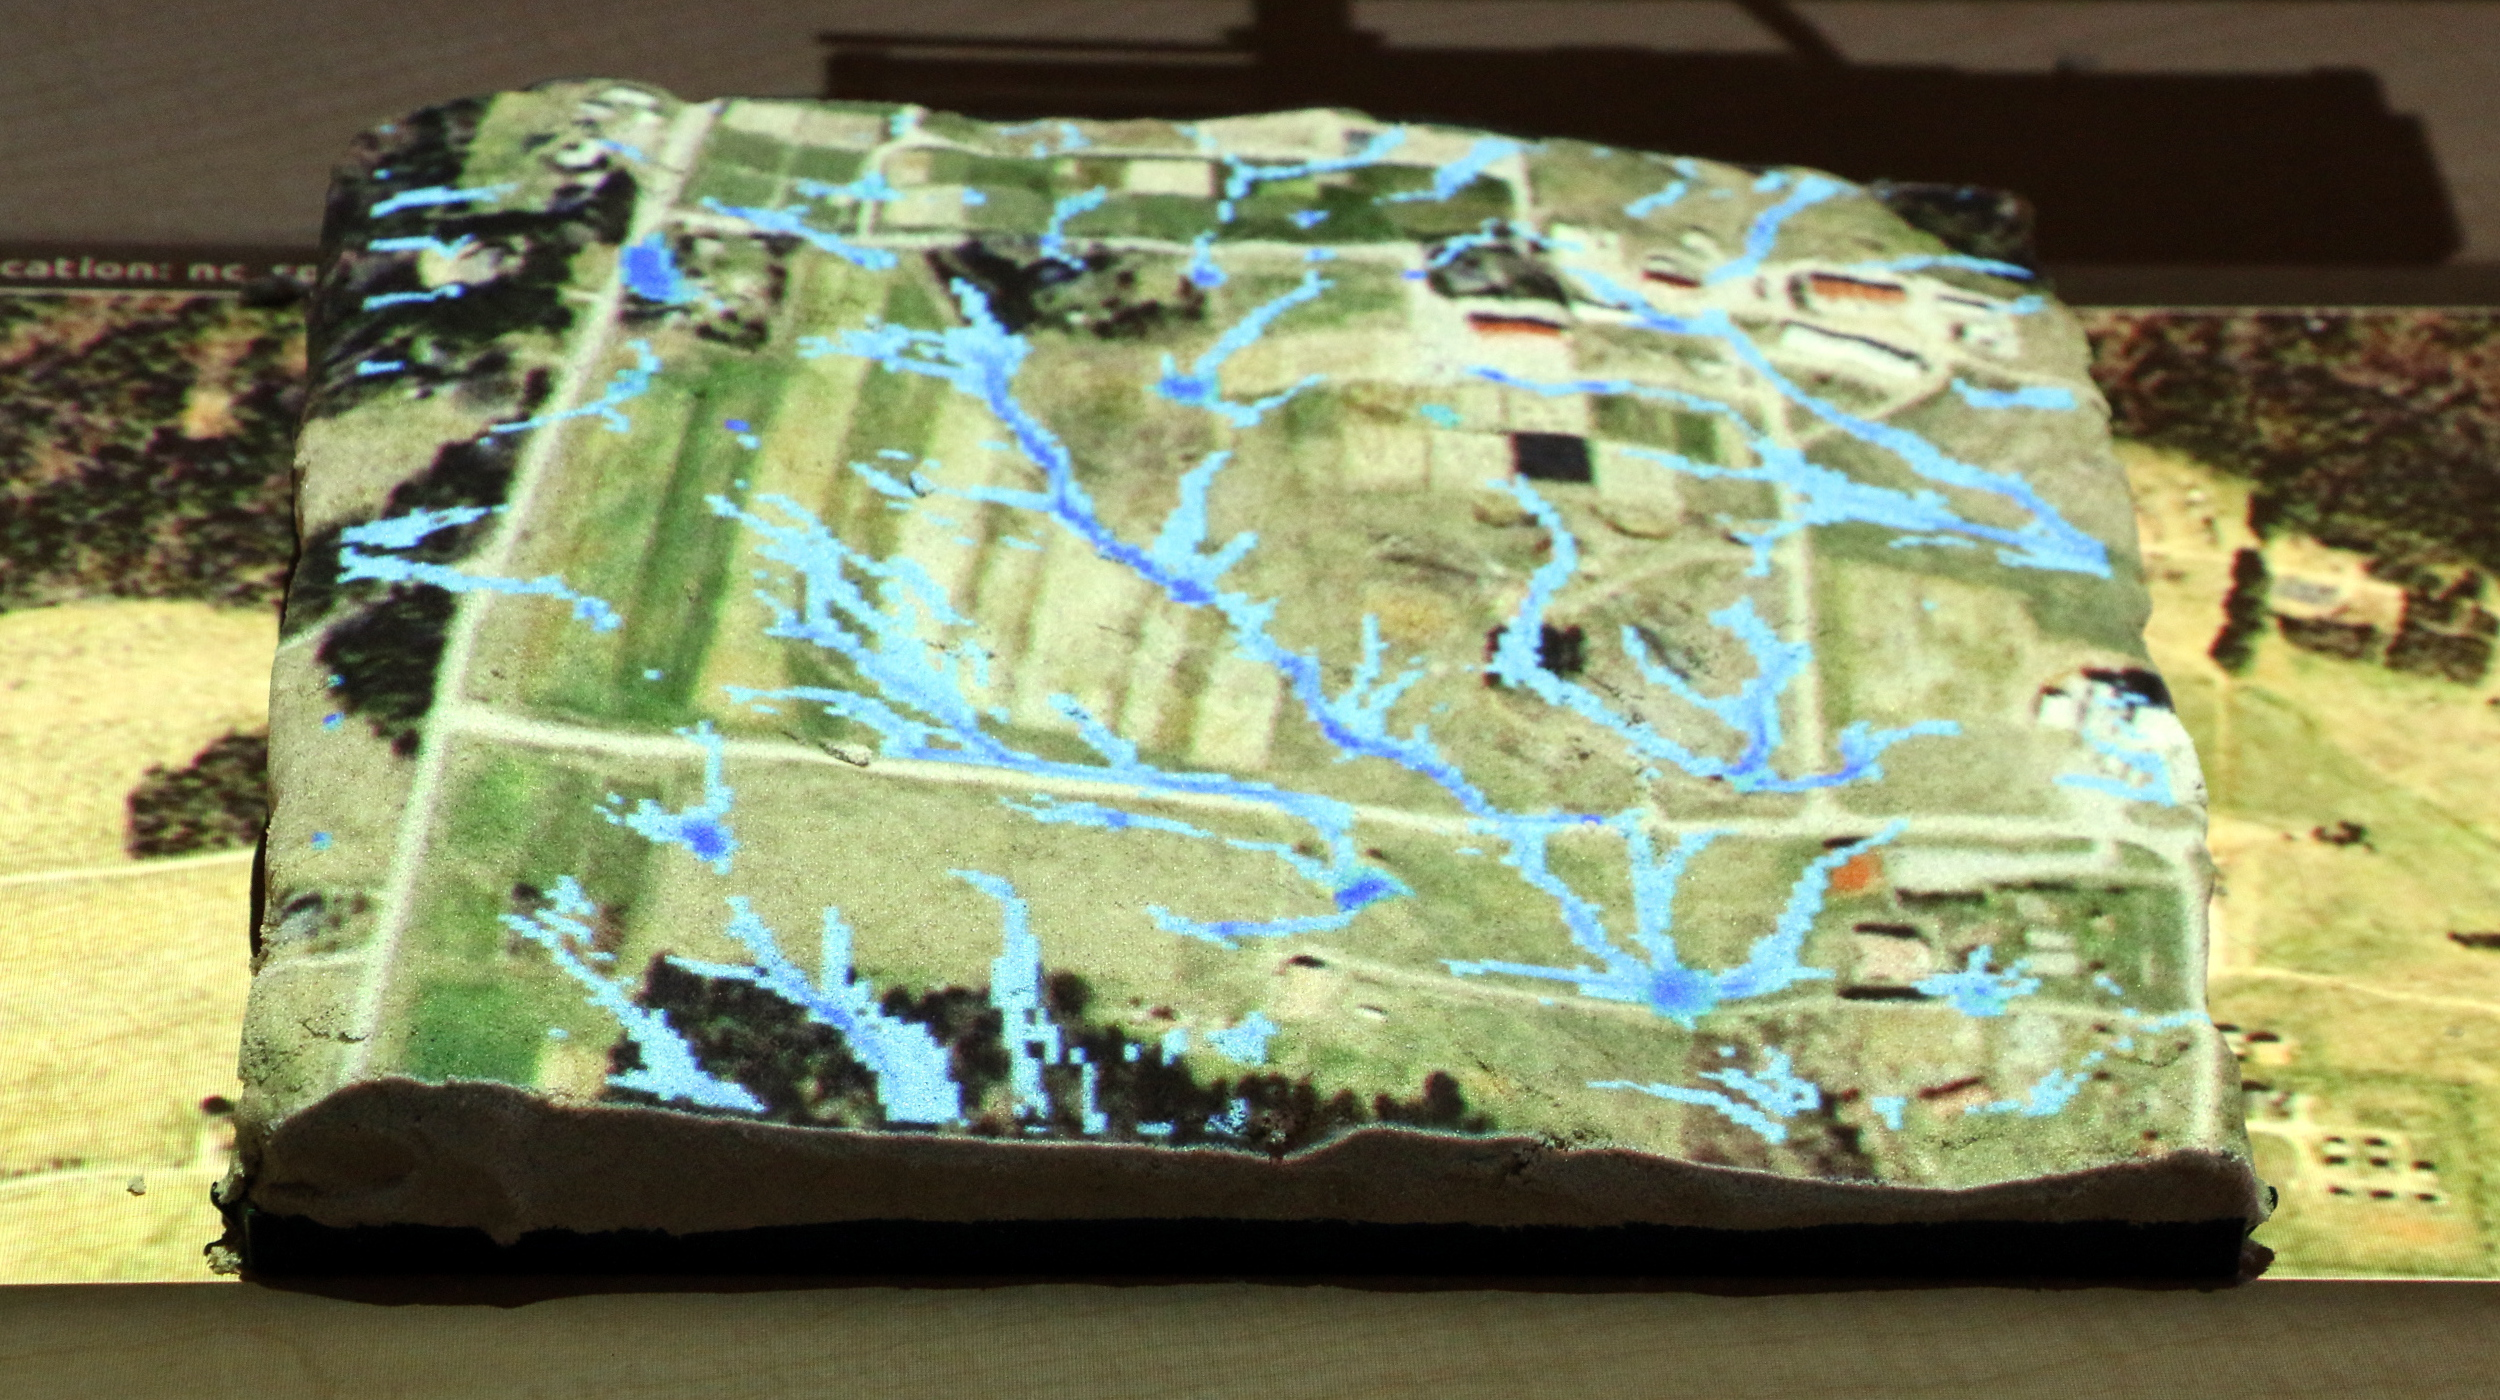
\includegraphics[width=0.32\textwidth]{images/tl_sequence_1.jpg}
		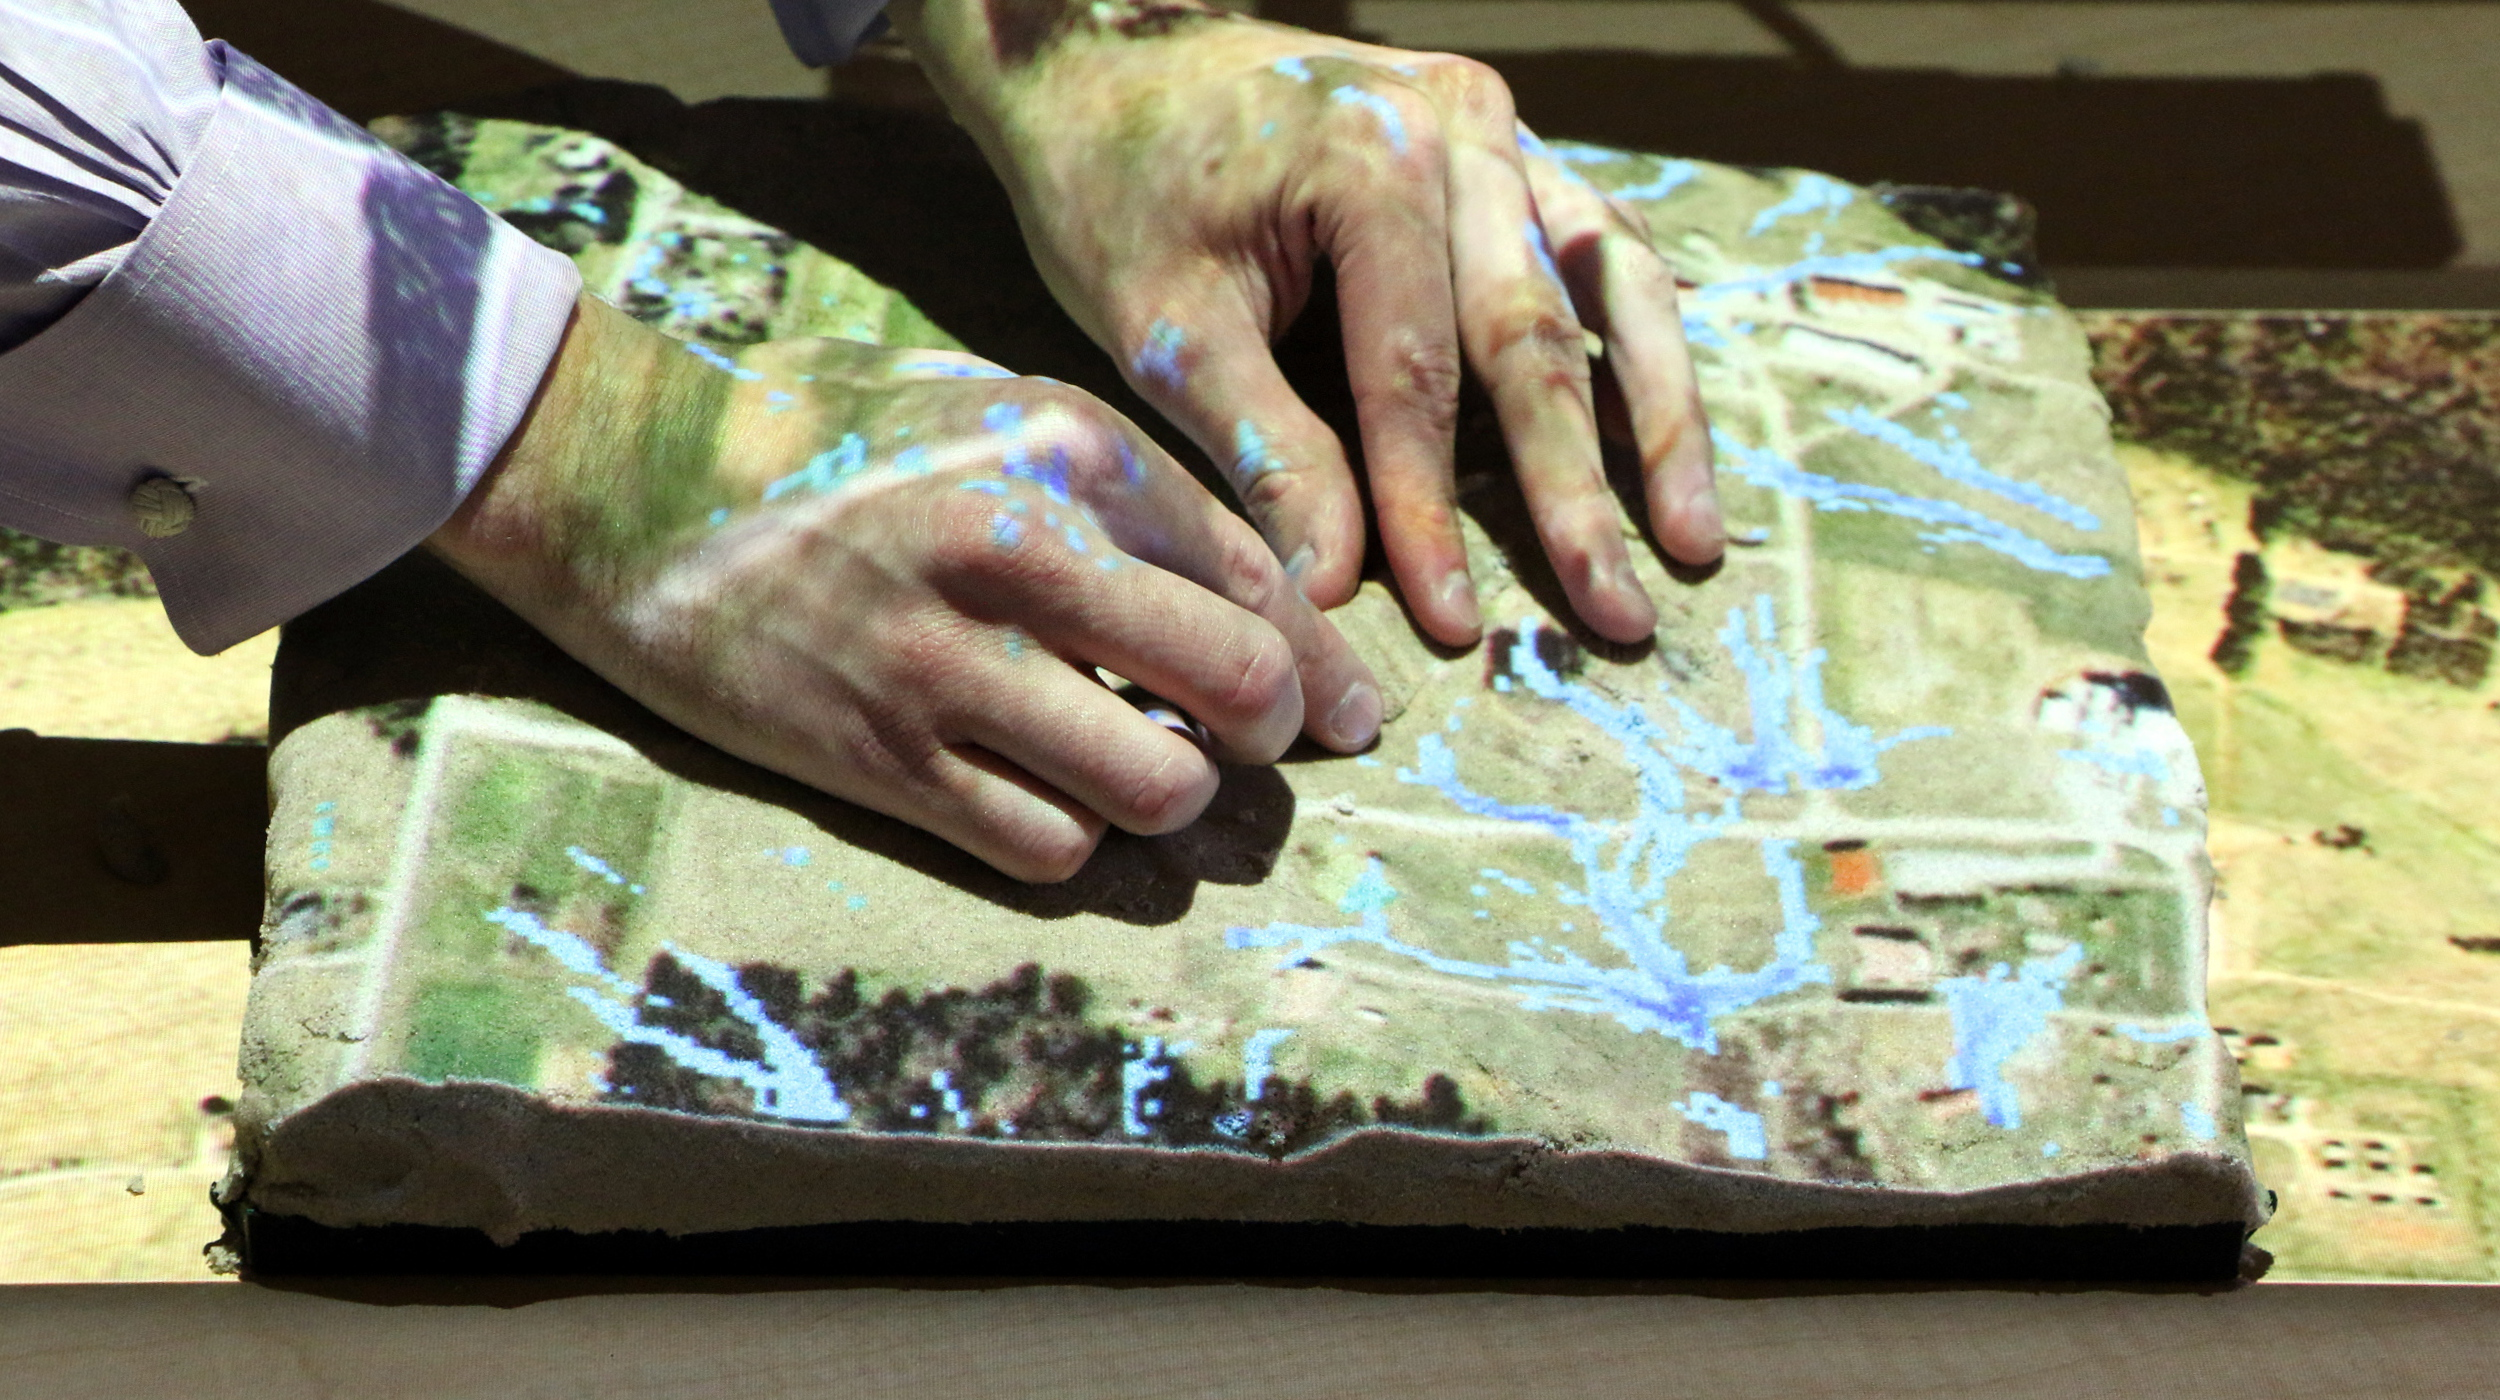
\includegraphics[width=0.32\textwidth]{images/tl_sequence_2.jpg}
		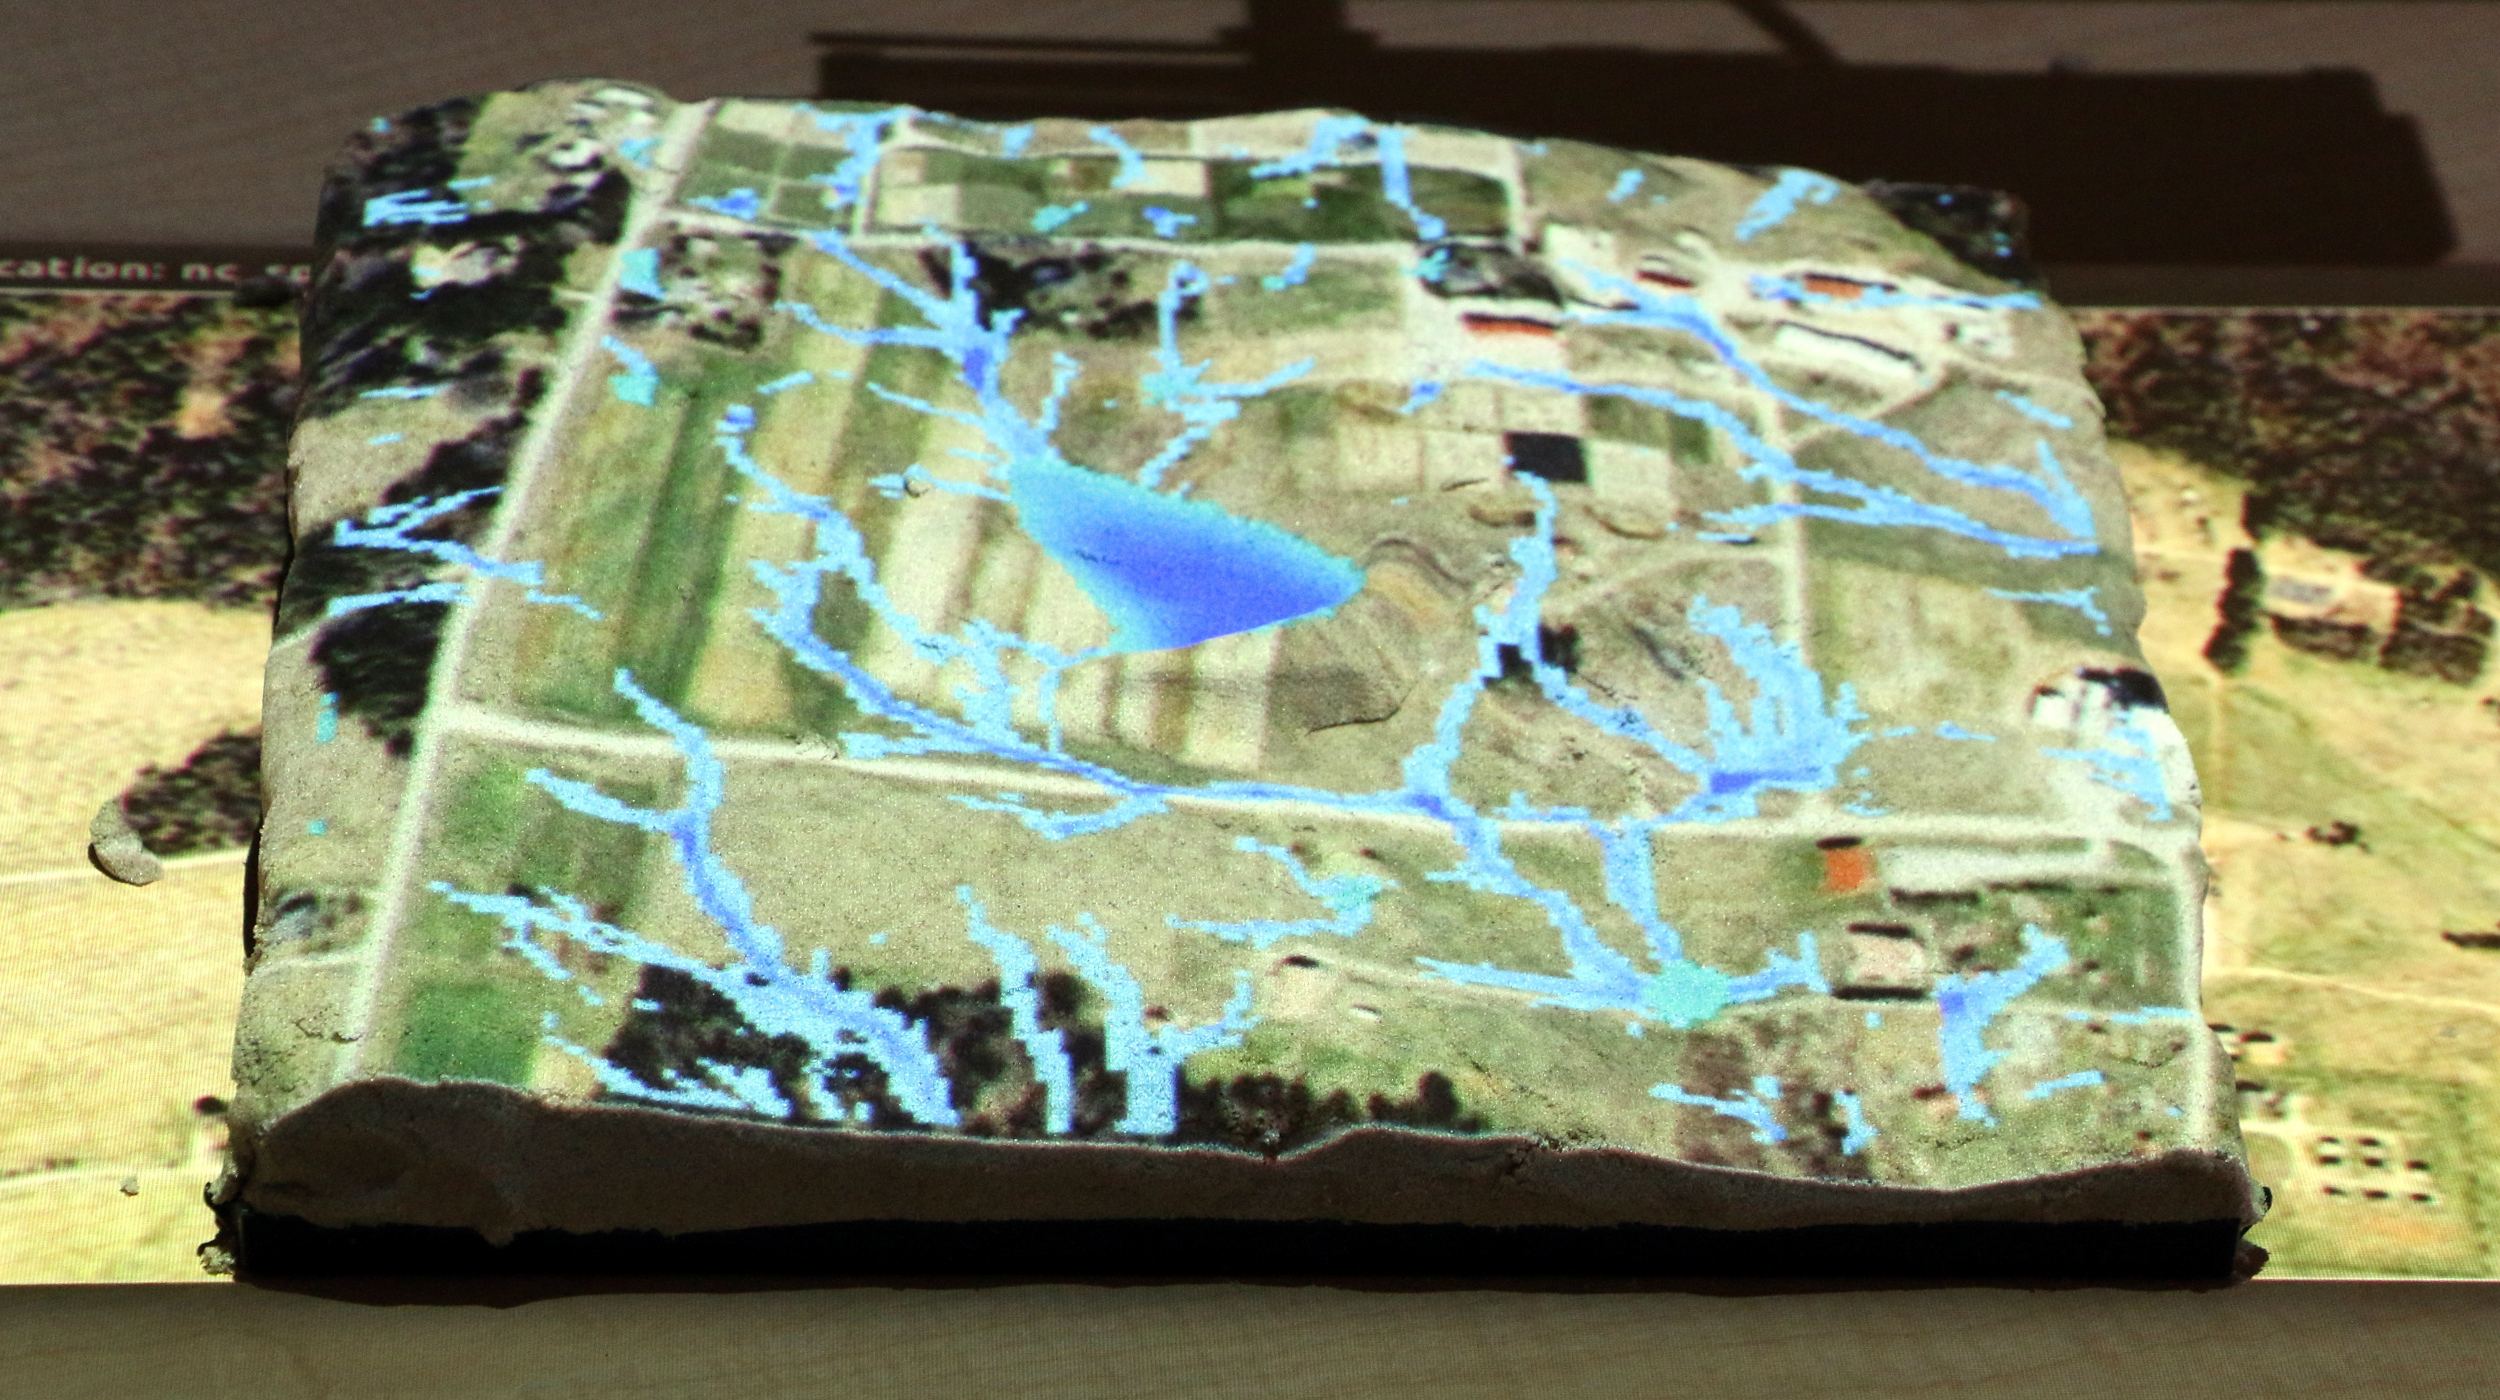
\includegraphics[width=0.32\textwidth]{images/tl_sequence_3.jpg}
	\caption{Tangibly modeling the flow of water with Tangible Landscape}
	\label{fig:tl_flow}
\end{center}
\end{figure*}

% A brief intro to TL

We present Tangible Landscape -- 
a tangible interface for geographic information systems (GIS). 
%
% challenge
Spatial thinking can be challenging --
it is multidimensional and 
can involve vast amounts of data. 
% computation
Spatial analyses and simulations, however, 
can be computed efficiently in GIS. 
%
% challenge of hci

\ldots

% tangible interaction
Tangible interfaces are designed to enable natural interaction with computers 
by physically manifesting data 
so that users can feel and manipulate it with their bodies. 
%
This means that people with little or no computer experience 
can intuitively, collaboratively explore data and scientific models and 
rapidly test ideas while learning from computational feedback. 
%
Through tangible interaction with GIS 
users can simulate, learn about, and design complex spatiotemporal processes naturally with their bodies while being situated in a collaborative, social context.
%
Tangible interfaces for GIS 
have the potential to fluidly, seamlessly combine
computational science with exploratory modes of creative thinking.
%


\ldots

(Fig.~\ref{fig:tl_flow})



% Concept diagram / illustration



\subsection{Spatial thinking and computation}

Spatial thinking -- `the mental processes of representing, analyzing, and drawing inferences from spatial relations' \cite{Uttal2013} -- is used pervasively in everyday life % at a personal scale 
for tasks like recognizing things, manipulating things, interacting with others, and way-finding. 
%
Spatial thinking is also used extensively in science, technology, engineering, the arts, and math 
for tasks like 
diagramming concepts, % \cite{Ormand2014}
visualizing data, % \cite{Ormand2014}
simulating physical processes,
mapping and manipulating molecules,
designing circuits, 
designing buildings, 
shaping sculpture,
and studying topology. 
%
Given the importance of spatial thinking -- personally, academically, and professionally -- %how can we improve it? 
how can we effectively improve our spatial performance, our ability to perform tasks that require spatial thinking? 
% how can spatial performance, our ability to perform tasks that require spatial thinking, effectively be improved?

Many spatial tasks can be performed computationally 
enabling us to efficiently store, model, and analyze large sets of spatial data 
and solve complex spatiotemporal problems.
%
In engineering, design, and the arts 
computer-aided design (CAD) and 3D modeling software are used to interactively, computationally model, analyze, and animate complex spatial forms. 
%
In scientific computing spatial patterns and processes can be mathematically modeled, simulated, and optimized. 
%
Geographic information systems, for example, can be used to computationally store, model, analyze, simulate, and represent geospatial patterns and processes. 
%
The open source 
Geographic Resource Analysis Support System (GRASS) GIS
for example supports 
`geospatial data management and analysis, image processing, graphics and maps production, spatial modeling, and visualization' \cite{GRASS}. 
%\footnote{\url{https://grass.osgeo.org/}} 
%
% add more citations

Computing mediates and transforms spatial thinking, expanding, but also constraining what is possible.
%
While spatial computing can augment spatial thinking 
-- distributing or offloading cognitive processes through digital computation -- 
the logic of implementation,
the limits of what is computationally possible, 
and the modes of input and output
constrain how we reason. % citations
%
Furthermore, 
when it is difficult to interact with a computer, 
to input commands and parse the resulting output, 
one has to think harder and risks frustration and demotivation. % citations (?)
% these cognitive costs and risks...
%
%Furthermore, 
%difficulty in interacting with a computer
%-- in inputing commands and parsing the resulting output --
%can add cognitive costs, generate frustration, and sap motivation. 

Unintuitive modes of human-computer interaction constrain thought and add cognitive and emotional costs. 
%
The paradigmatic modes for interacting with computers today 
-- command line interfaces (CLI) and
graphical user interfaces (GUI)
%including touch interfaces
 -- 
require physical input from devices like keyboards, mice, digitizing pens, and touch screens, but
output %present %render
data visually as text or graphics. 
%
Theoretically this disconnect between intention, action, and feedback should make interaction less intuitive \cite{Dourish2001,Ishii2008}. 
%
Furthermore, it can be challenging to parse data that is only presented visually. 
Spatial data -- especially 3D spatial data -- presented graphically can require sophisticated spatial reasoning skills such as mental rotation \cite{Shepard1971}, spatial visualization, and spatial perception \cite{Linn1985} to parse and understand, much less manipulate.

% digital technologies mediate spatial thinking

% how do they affect spatial performance?

% what technologies are most effective?


\subsection{Tangible interaction}

Tangible interfaces -- interfaces that couple physical and digital data \cite{Dourish2001} -- 
are designed to physically manifest digital data so that we can cognitively grasp and absorb it,
so that we can think with it rather than about it \cite{Kirsh2013}. 
%
Ishii and Ullmer envisioned that tangible interfaces would  `take advantage of natural physical affordances to achieve a heightened legibility and seamlessness of interaction between people and information' \cite{Ishii1997}. 
%
With a tangible interface both input and output are physical. 
%
Data can be felt as well as seen; data can be directly, physically manipulated, leveraging highly developed motor skills. 
%
Thus intention, action, and feedback should be seamlessly connected 
enabling automatic, subconscious, and intuitive interaction.
%%%

Tangible interfaces let users interact with computers while (functionally) thinking with their bodies. 
%
By thinking with their bodies, by embodying cognition 
users may be able to reduce their cognitive loads by
offloading cognitive tasks like 
spatial perception and manipulation 
onto the body and 
physically simulating processes.
%
In embodied cognition higher cognitive processes are grounded in, built upon, and mediated by bodily experiences such kinaesthetic perception and action \cite{Hardy-Vallee2008}. 
%
When people use tools they temporarily, contingently incorporate them into their body schema, feeling the perimeter, weight, and balance of the tool, 
sensing resistance when the tool touches something, 
as if the tool was an extension of the body \cite{Maravita2004}.
%
Because tools can be cognitively gripped and absorbed in ones body schema, they mediate embodied cognition -- affording new bodily experience and action and thus extending ones capacity for thought. 
%
Tangible interfaces are designed to make computation tangible so that it can be cognitively gripped and absorbed, so that computation can be understood with the body.
%%%

It can be challenging and cognitively taxing to visually perceive and parse space, to for example visually judge distances and imagine volumetric form.
%
Distance and physical properties like size, shape, volume, weight, hardness, and texture, however, can be automatically and subconsciously assessed kinaesthetically with the body \cite{Jeannerod1997}. 
%
By affording physical feedback tangible interfaces should, therefore, reduce the cognitive load needed to judge spatial distances, relationships, patterns, and forms. 

Furthermore, some cognitive processes can be physically simulated, offloading the cognitive work onto the body \cite{Kirsh2013}. 
%
% Examples of physical simulation
%
%Dancers for example use marking 
%-- a simplified, abstraction of a dance phrase -- to learn and practice elements or aspects of the phrase. 
%Marking is 
%a model 
%a sketch-through-action
%\cite{Kirsh2013}



%
Architects massing models
Office of Metropolitan Architecture
foam massing models 
\cite{Yaneva2009}
%
or Frank Gehry's creative process of thinking through the movement of gestural drawing and exploratory form finding with massing models
\cite{Gehry2004,Pollack2006}
%

Professionals like designers develop creative ideas through `reflection-in-action,' 
an iterative, exploratory process 
of framing the problem, ideation or making, and critical reflection \cite{Schon1983}.
This exploratory process may unfold in an instant in action, 
repeated continually through acts like drawing or model making. 
%
Frank Gehry for example develops his designs through exploratory form finding with massing models
and by thinking through the movement of gestural drawing
\cite{Gehry2004,Pollack2006}.

An ethnography of the Office of Metropolitan Architecture
showed that architects in the firm used practices like reuse, adaption, and exploratory modeling
to develop designs through iterative processes \cite{Yaneva2009}. 
The architects, for example, explored form by carving foam massing models with hot-wire cutters, reflecting on each model as they carved, while building up a library of forms. Ideas and forms set aside and unused in one project might show up in other projects, recycled and adapted \cite{Yaneva2009}.


%
When tangible interactions are designed to be analogous to everyday, physical tasks 
like unscrewing a bottle top \cite{Kirsh2013}, picking up and placing objects, or sculpting sand...
users may already understand what to do. 
Such interaction should be highly intuitive, drawing on existing motor schema and cultural knowledge. 
%

%Embodied cognition 
%enables 
%exploratory
%trial and error process
%
%generative intention, enaction, feedback 
%rapid cycles
%
%Especially powerful for 
%generative processes
%like form finding
%
%
%
%Cognition and interaction are embodied.
%
%
%Tangible interfaces 
%
%...
%simply by affording kinaesthetic, physical feedback as well as visual feedback 
%
% discuss creative design process & computationally enhanced creative design process (later perhaps?)


%In a seminal paper Ishii and Ullmer envisioned tangible user interfaces that would 
%`bridge the gap between cyberspace and the physical environment by making digital information (bits) tangible' \cite{Ishii1997}.
%They described `tangible bits' as `the coupling of bits with graspable physical objects' \cite{Ishii1997}. 


% embodied cognition


% By affording kinaesthetic, physical feedback as well as visual feedback 

%If a tangible interface is well designed and the interactions are analogous to 
%The process of interaction is 



... \\
	
	%Affordance
	
		% physical i/o 
	
		% physical / kinaesthetic as well as visual feedback

% Embodied spatial thinking

	%Understanding space with ones body

	%What is embodied spatial thinking?

	%Cognitive offloading through physical simulation


% Diagram of disconnect between intention, action, and feedback in GUI
% VS coupling of intention, action, and feedback in a TUI


%
%% embodied spatial thinking
%
%% embodied cognition
%Embodied cognition highlights the importance of a kinaesthetic, pragmatic understanding of space
%and the enaction of spatial transformation -- for the act of transforming an object changes how we think about space. 
%As Kirsh argues, sometimes `we know more by doing than by seeing' \cite{Kirsh2013}.
%%
%% embodiment in STEM
%Embodied spatial thinking may lead to improvements in STEM performance by reducing cognitive loads with pragmatic representations and physical simulation and by enhancing perception with visual and haptic feedback. 
%%
%Embodied and computationally enriched cognition may enhance spatial thinking in novel ways
%enabling and encouraging coupled creative and analytic the.
%
%

\subsection {Aim and objectives}
%OR
\subsection{Research questions}

\pagebreak


\section{Methodology}
\subsection{Tangible Landscape}

\paragraph{Concept}
%
Tangible interfaces for GIS 
should ease the cognitive burden of 
visualizing, interacting with, reasoning about space
by giving spatial data an interactive, physical form 
that users can cognitively grasp and kinaesthetically explore. 
%
Tangible Landscape -- a tangible user interface for GRASS GIS --
couples a physical and digital model of a landscape through a continuous cycle of 3D scanning, geospatial modeling, and projection
so that users can intuitively interact with the modeled landscape in near real-time.
%
Conceptually Tangible Landscape physically manifests geospatial data 
so that users can hold a GIS in their hands -- 
so that they can, for example, feel the shape of the earth, sculpt its topography, and direct the flow of water with their hands.
%
It enables users to 3D sketch -- 
to naturally model forms such as topography, 
draw points and polygons, 
and interact with simulated physical processes -- 
in a rapid, iterative process 
of observation, hypothesis generation and testing, and inference. 
%
Tangible Landscape is meant to fluidly, seamlessly combine
computational science with exploratory modes of creative thinking.

\paragraph{Evolution}
%
Tangible Landscape evolved from 
Illuminating Clay \cite{Piper2002a} and 
the Tangible Geospatial Modeling System (TanGeoMS) \cite{Tateosian2010}. 
%
% Illuminating Clay
Illuminating Clay coupled a clay model and digital model of landscape 
through a cycle of laser scanning, spatial modeling, and projection.
%
By enriching physical models of urban spaces and landscapes 
with spatial analyses  
such as 
elevation, aspect, slope, cast shadow, profile, curvature, 
viewsheds, solar irradiation, and water direction
it enabled
intuitive form-finding, 
streamlined analog and digital workflows, 
and enabled multiple users to simultaneously interact in a natural way \cite{Ratti2004}. 
%
Illuminating Clay had a very limited library of custom implemented spatial analyses. 
%
Since many of analyses were adapted 
from the open source GRASS GIS project \cite{Piper2002a} 
there was a call to integrate it with GRASS GIS 
in order to draw on GRASS GIS's extensive libraries 
for spatial computation \cite{Piper2002b}. 
%
The effort to couple a physical landscape model with GRASS GIS \cite{Mitasova2006} 
led to the development of 
TanGeoMS \cite{Tateosian2010}.
%and then Tangible Landscape  \cite{Petrasova2014,Petrasova2015}.
%
% Tangible Geospatial Modeling System
TanGeoMS coupled a physical model and GIS model of a landscape 
through a cycle of laser scanning, geospatial computation in GRASS GIS, and projection
giving developers and users assess to 
%drawing on 
a sophisticated library for 
spatial modeling, simulation, visualization, databasing.
%
It enriched freeform hand modeling with geospatial simulations like diffusive water flow and erosion-deposition 
so that users could easily explore how 
changes in topographic form affect landscape processes. 
%
% Augmented Reality Sandbox
Tangible Landscape -- the next generation of this system -- was inspired by
the open source Augmented Reality Sandbox \cite{Kreylos2012}
which couples a sandbox with a digital model of a landscape 
through a real-time cycle of 3D scanning with a Kinect sensor, spatial modeling and simulation, and projection.
%
% TL
While TanGeoMS used an expensive terrestrial lidar scanner for 3D scanning \cite{Tateosian2010}, 
Tangible Landscape uses a low-cost 3D sensor like the Kinect 
for real-time depth and color sensing. 
%
The \nth{1} generation of Tangible Landscape \cite{Petrasova2014} 
used the \nth{1} generation Kinect with structured light sensing \cite{Smisek2011}, 
and the \nth{2} generation of Tangible Landscape \cite{Petrasova2015} 
used the \nth{2} generation Kinect with time-of-flight sensing \cite{Bamji2015} . 

\paragraph{Design}
Tangible Landscape was designed to let users naturally explore 
spatial data, models, and simulations in an engaging, playful way
by 3D sketching (Fig.~\ref{fig:subsurface}).
%
As users sculpt the physical model
the model is 3D scanned as a point cloud, georeferenced, imported into GIS, 
and either binned or interpolated as a digital elevation model. 
The digital elevation model is used to compute 
geospatial analyses, models, and simulations, 
which are then projected back onto the physical model 
-- all in near real-time (Fig.~\ref{fig:system_schema}). 
%
This enables users to tangibly interact with digital models and simulations
either by shaping topography with their hands or 
by placing markers that are identified through object detection. 
%
As the digital models and simulations update
the results are projected back onto the model for the users to see. 

Because the model is continually scanned
users hands will be digitized as they sculpt or place objects. 
%
Scanning users' hands as topography can be distracting; 
it also, however, helps users understand how the system works
-- by seeing how direct interaction is --
and encourages play. 
Users can, for example, cup their hands over the model 
and see them fill with simulated water. 

% implementation

%Tangible Landscape was implemented as a plugin for GRASS GIS...
% get text from Anna?


\begin{figure}[h!]
\begin{center}
		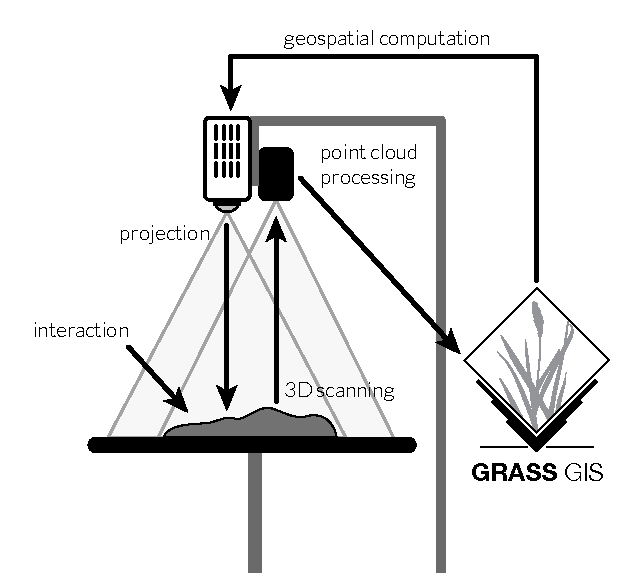
\includegraphics{images/system_schema.pdf}
	\caption{How Tangible Landscape works: a near real-time feedback cycle of interaction, 3D scanning, point cloud processing, geospatial computation, and projection}
	\label{fig:system_schema}
\end{center}
\end{figure}

\begin{figure*}[h!]
\begin{center}
		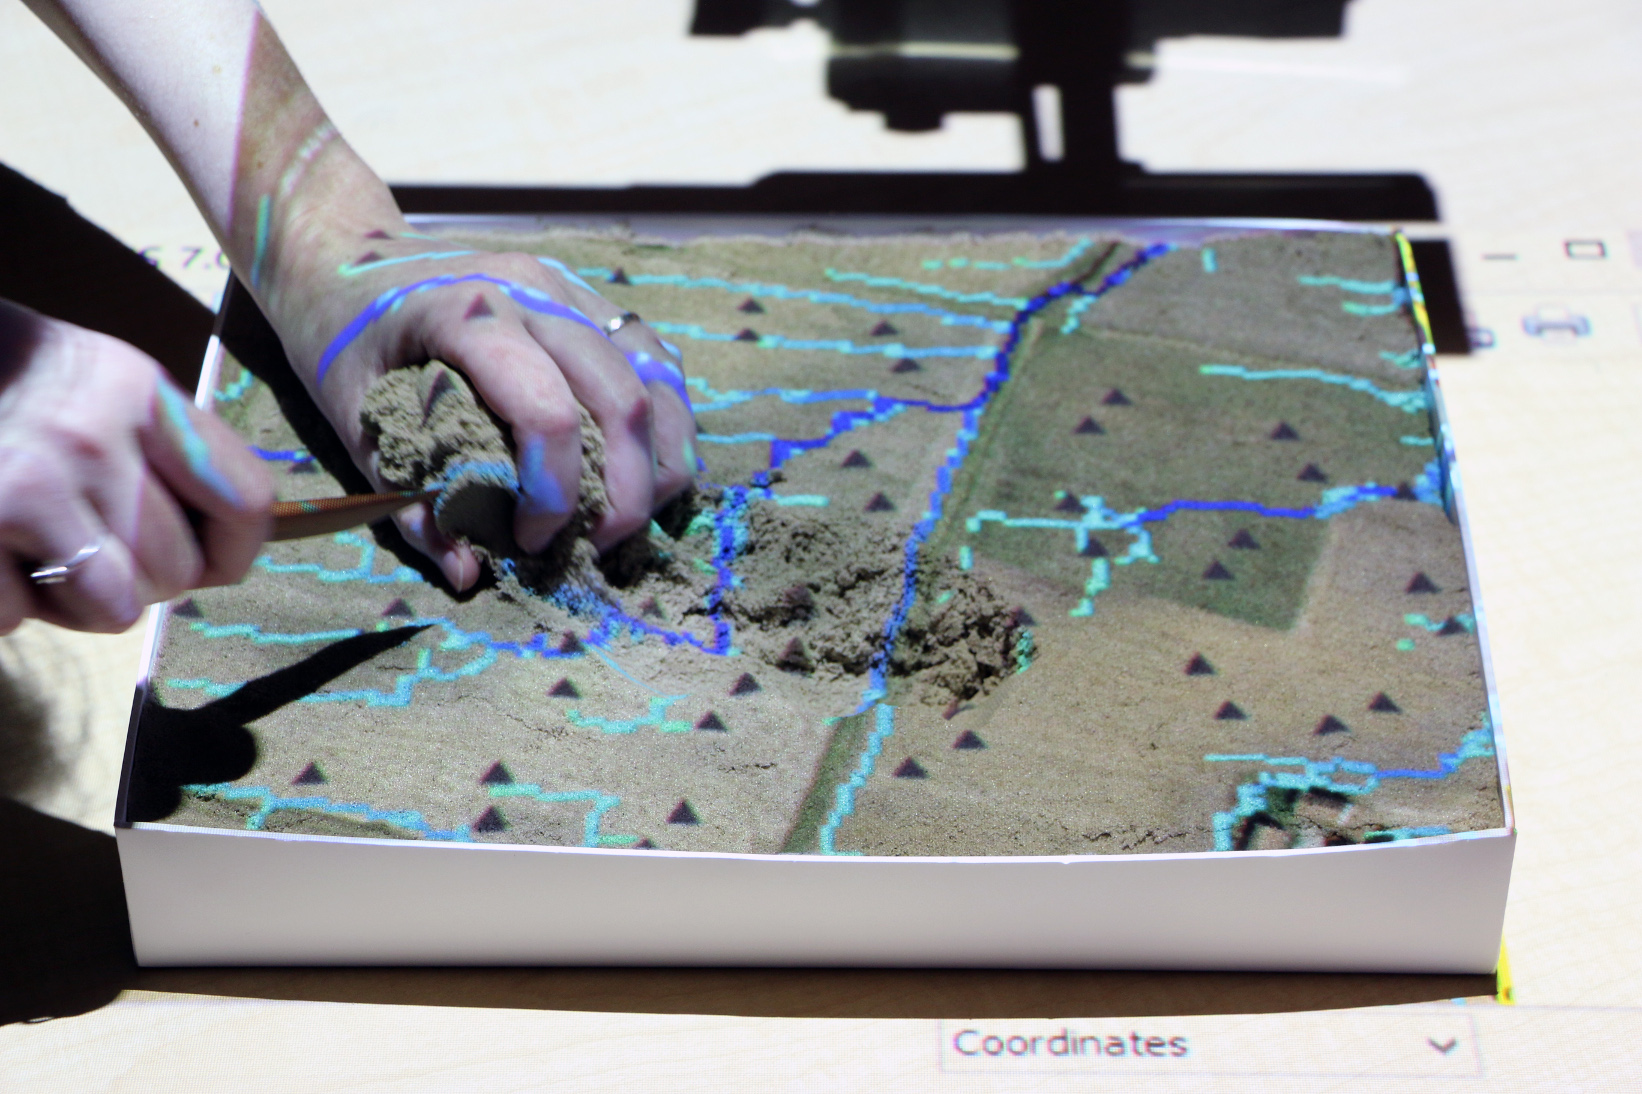
\includegraphics[height=65px]{images/subsurface_1.jpg}
		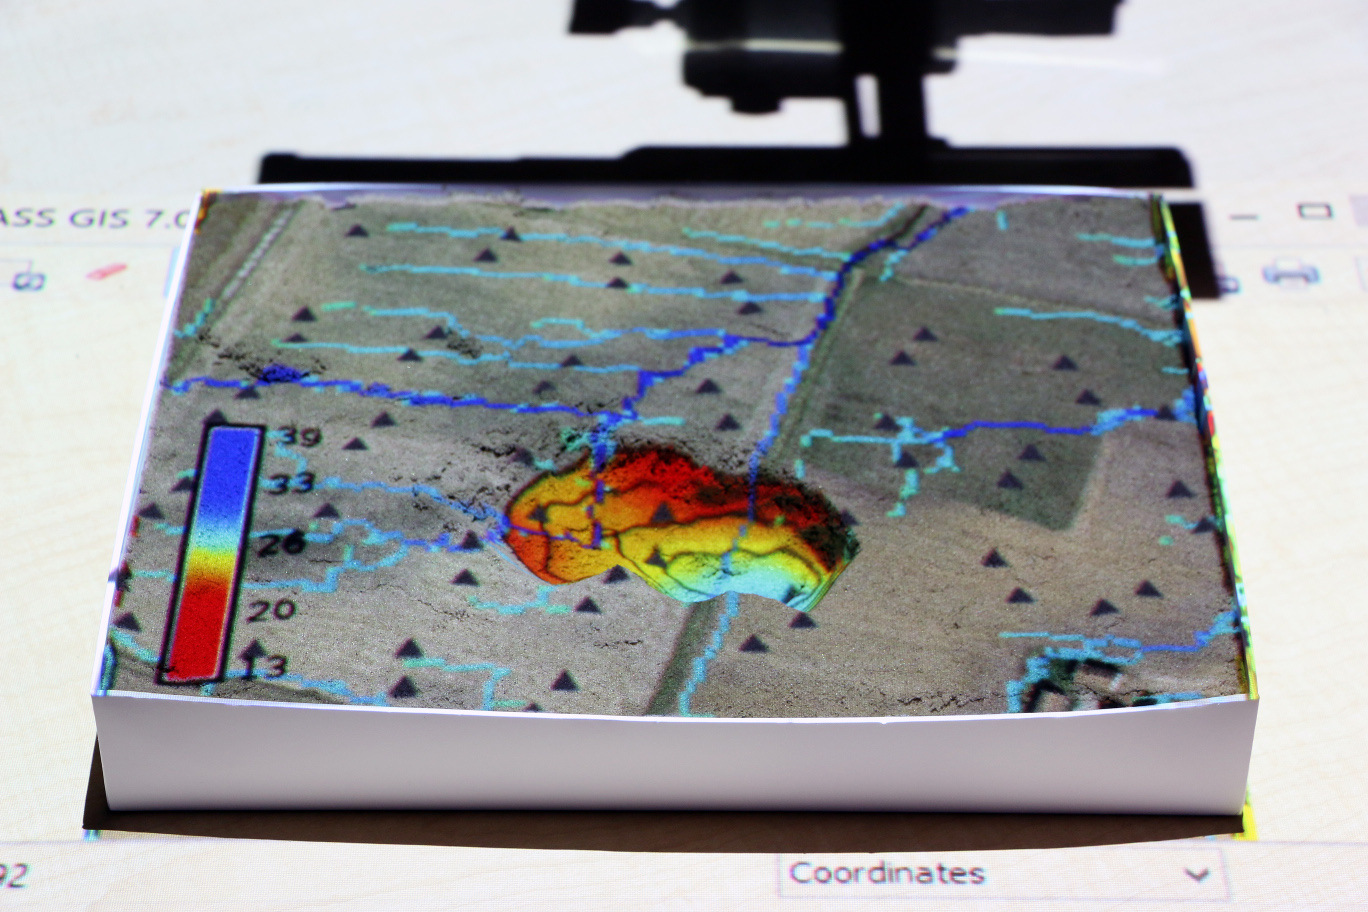
\includegraphics[height=65px]{images/subsurface_2.jpg}
		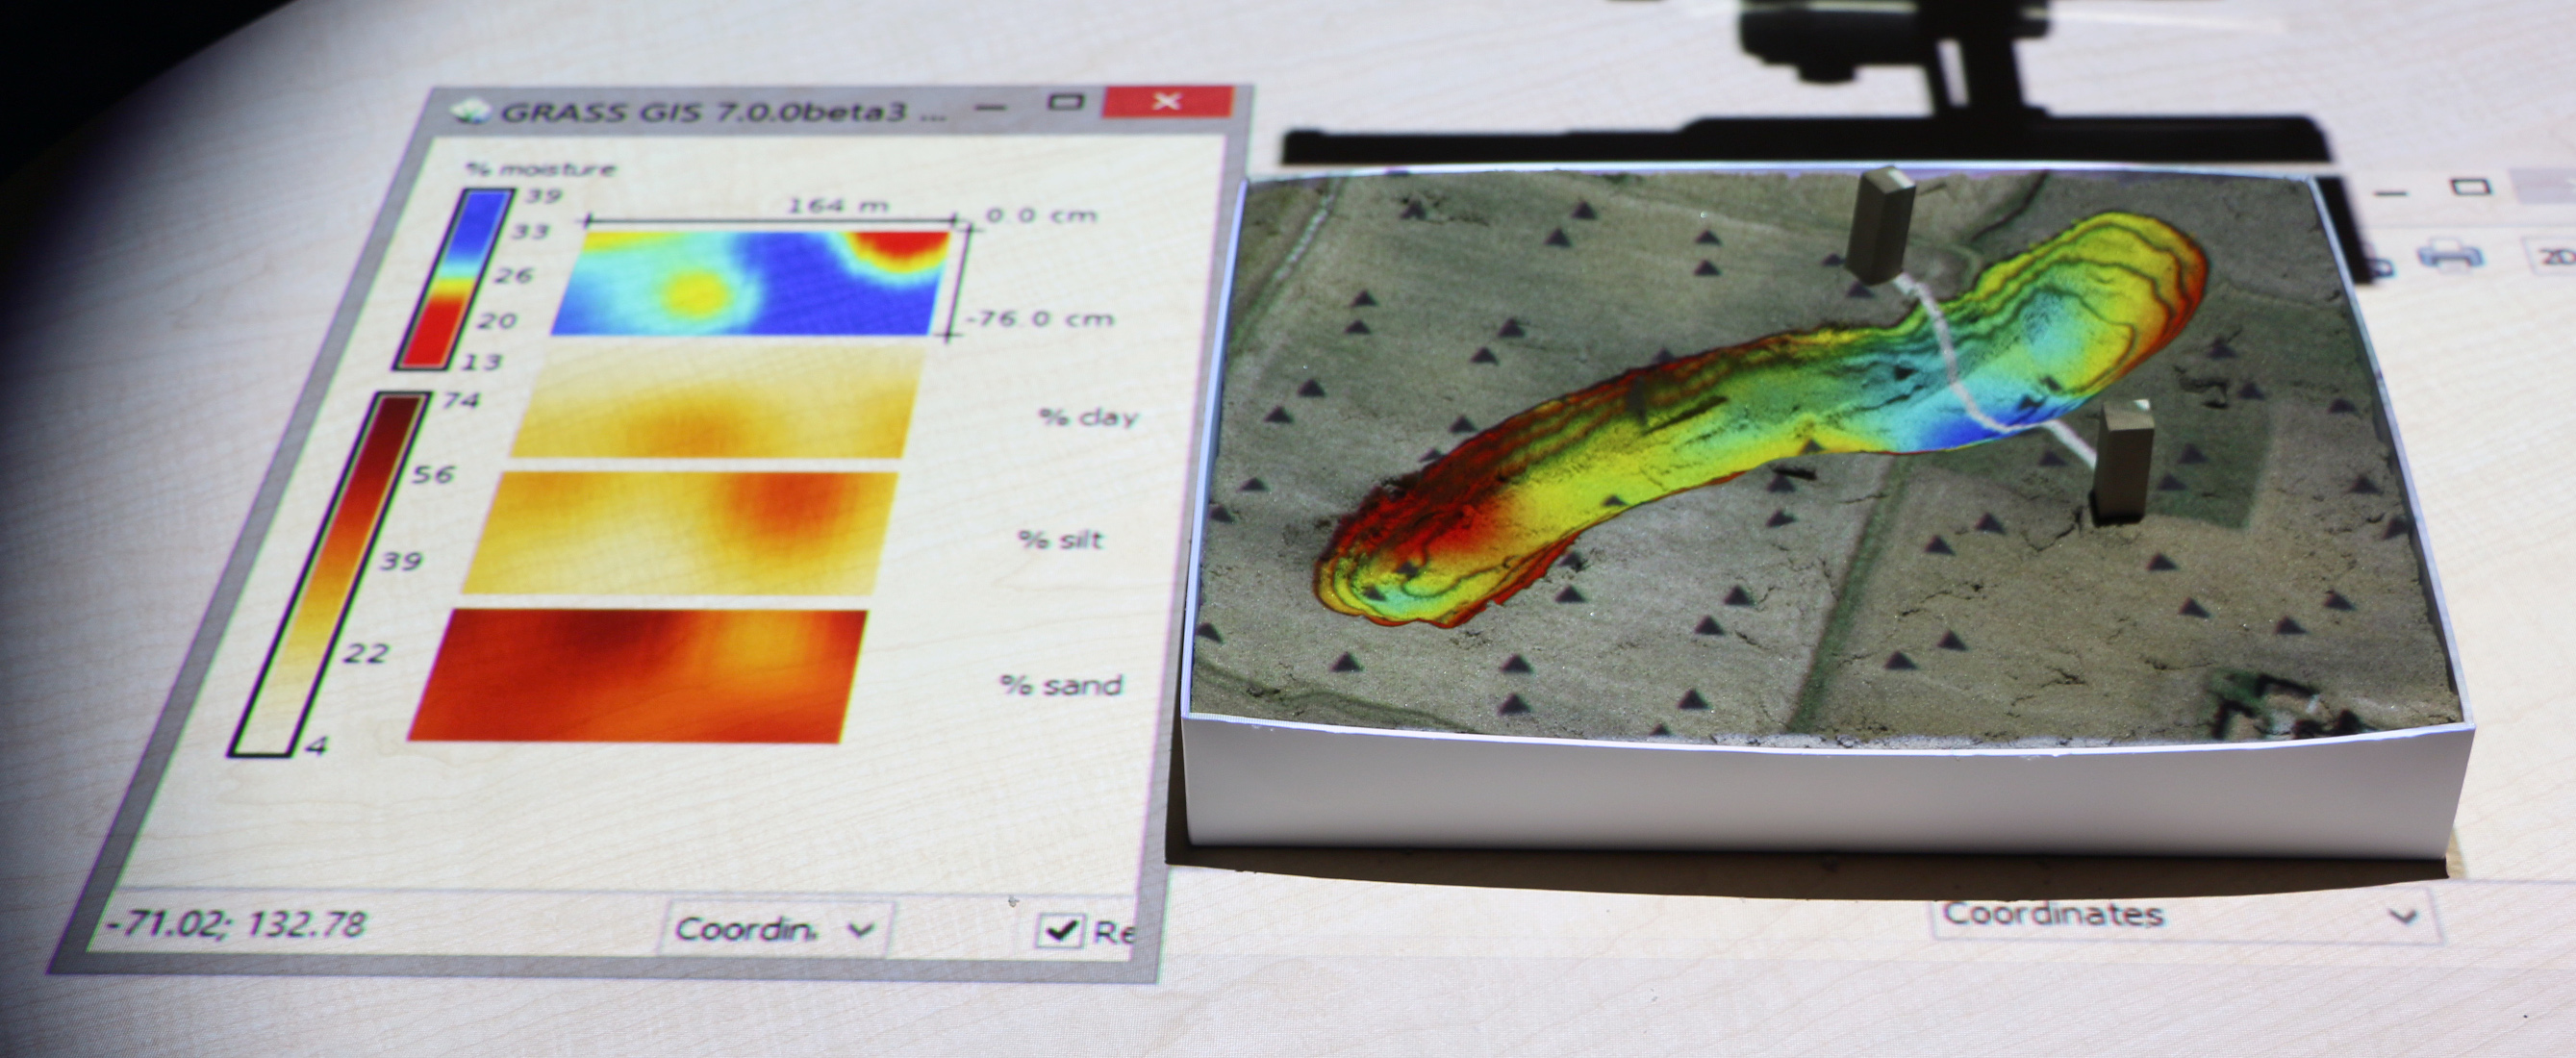
\includegraphics[height=65px]{images/subsurface_3.jpg}
	\caption{Naturally exploring subsurface soil moisture and soil types with Tangible Landscape}
	\label{fig:subsurface}
\end{center}
\end{figure*}

%-------------BOOK-------------------
%was designed to intuitively 3D sketch landscapes.
%This continuous shape display is more tightly integrated with
%GRASS GIS and has new modes of interaction based on
%object recognition so that users cannot only sculpt,
%but also sketch in 3D -- rapidly exploring ideas while learning from near real-time feedback.
%Tangible Landscape is more affordable than its predecessors because it uses
%a Kinect sensor to 3D scan physical models.
%As a continuous shape display with object recognition a wide range of media can be used
%such as polymer-enriched sand, clay, 3D prints, CNC-machined models, and architectural models.
%It is more tightly integrated with GIS, using a GRASS GIS plugin to automatically scan, process,
%georeference, import, and analyze the model.
%Because it is so tightly integrated with GRASS GIS users can also use the GUI, the command line,
%and scripting as advanced controls for tasks not suited to
%a tangible user interface.




\paragraph{Fabrication}

% Fabrication and materiality
The physical model is often made of polymer-enriched sand so that users can easily sculpt forms in a medium that will hold its shape, has good plasticity, and has a familiar feel and aesthetic. 
% model making, digital fabrication, CNC, 3D printing, molding and casting, etc



% materiality

%
Tangible Landscape 
typically uses familiar, everyday materials -- like sand and wooden blocks -- for modeling. 
%
Interactions -- sculpting sand and moving wooden blocks -- 
are analogous to everyday tasks
so users should subconsciously knows what to do and how to do it, 
leveraging existing sensorimotor schemas. 
%
The materiality -- the feel, look, and physics -- of the media matters. 
The choice of material can afford different interactions
and mediate meaning, emotion, and motivation. 
%
We typically use a polymer-enriched sand for the physical model
so that users can easily sculpt forms in a medium 
that will hold its shape, has good plasticity, and has a familiar feel and aesthetic. 
%
Because polymeric sand can easily be cast in molds and will be hold its form, 
we use computer-numeric control (CNC) machined or 3D printed molds to
cast polymeric sand into precise models (Fig.~\ref{fig:casting}.

\begin{figure*}[h!]
\begin{center}
		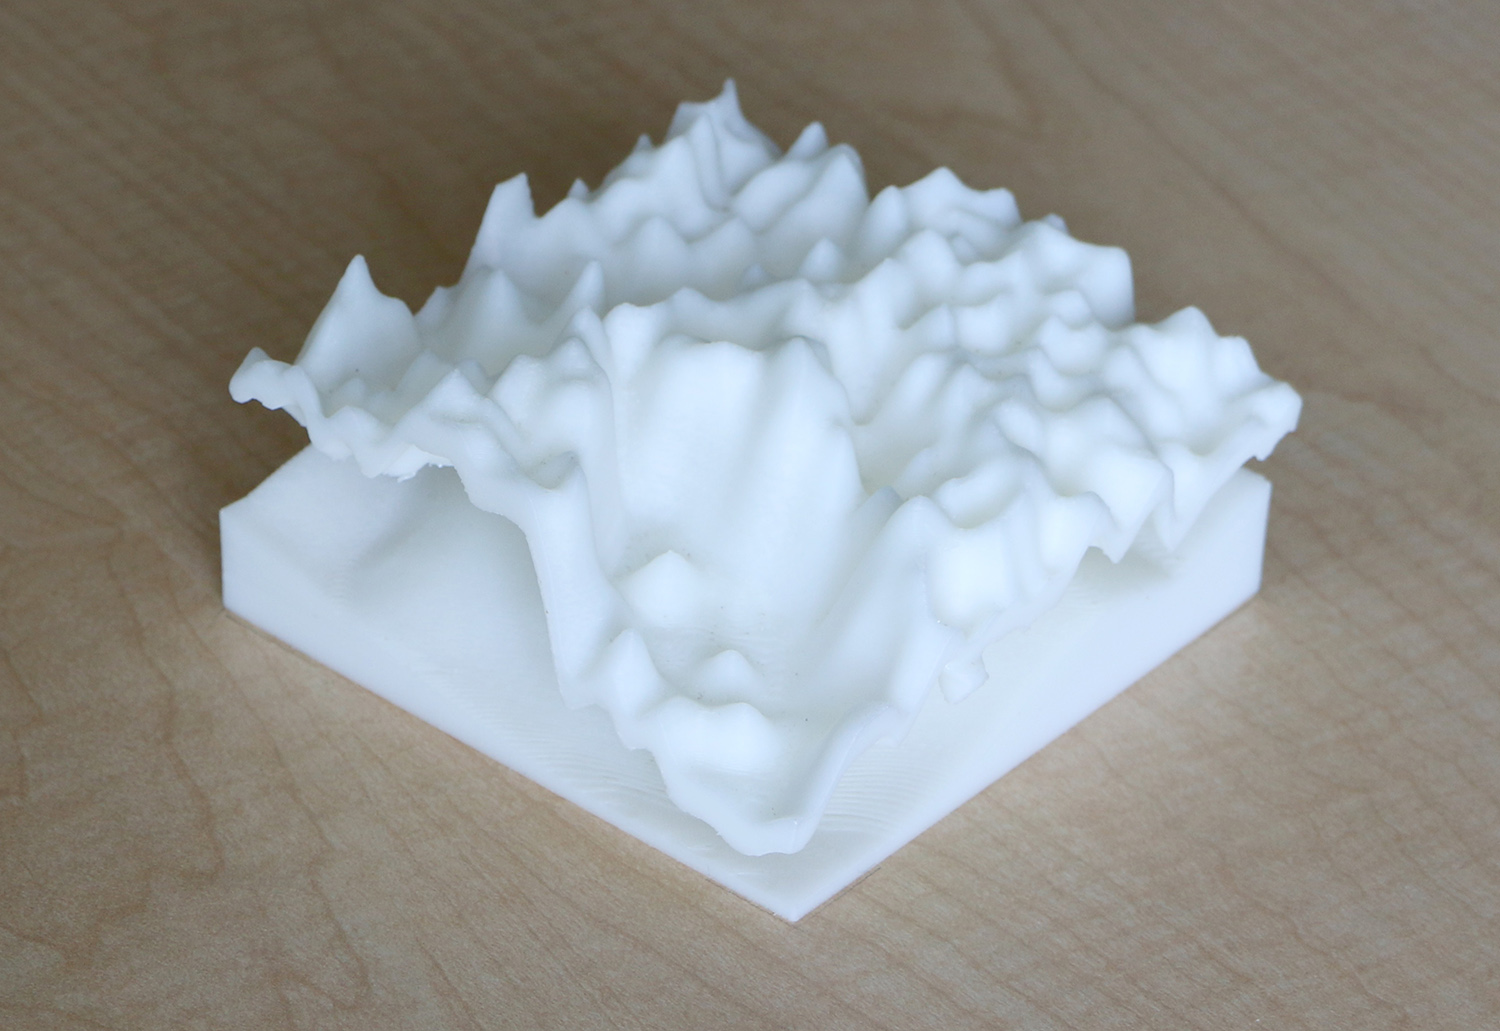
\includegraphics[width=0.3\textwidth]{images/3d_print_1.jpg}
		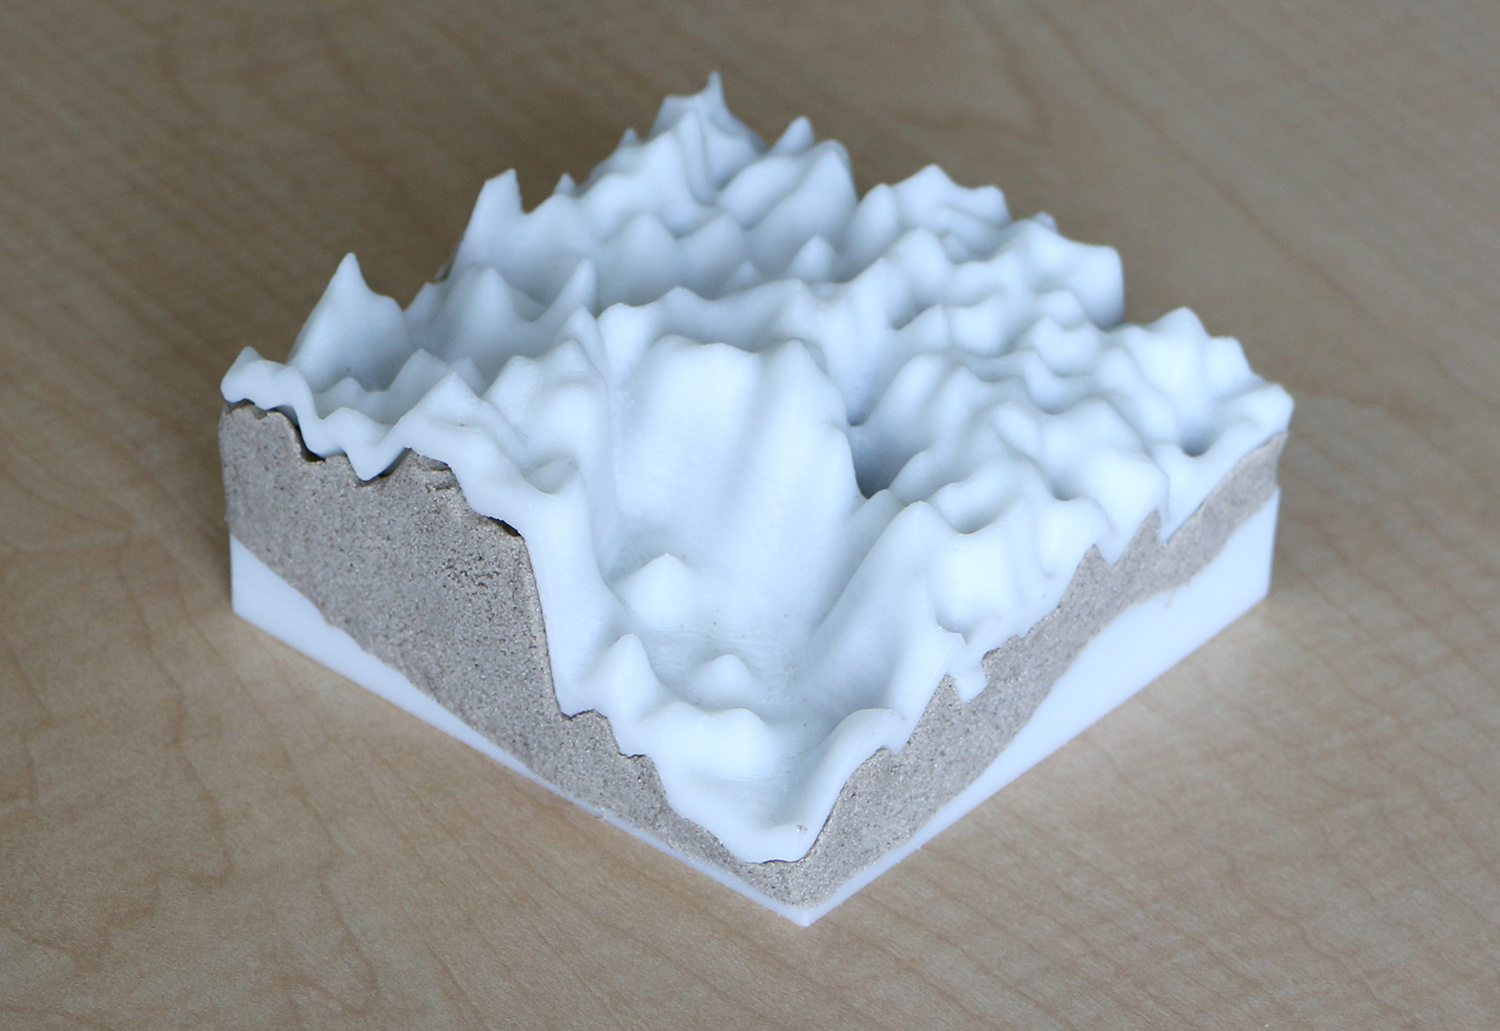
\includegraphics[width=0.3\textwidth]{images/3d_print_2.jpg}
		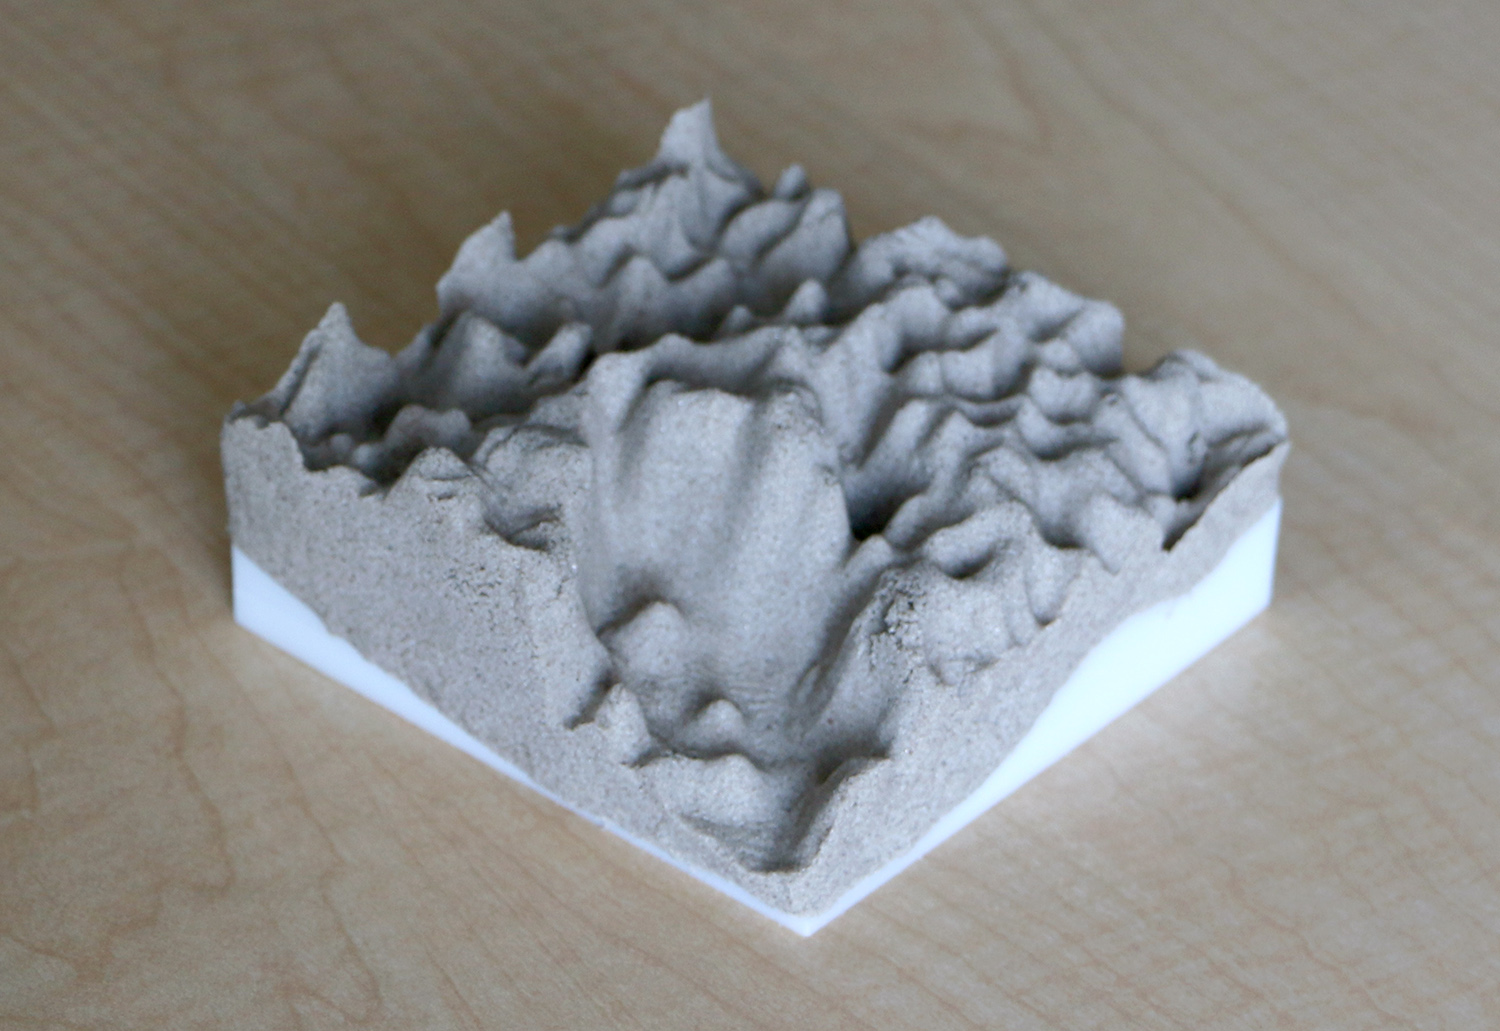
\includegraphics[width=0.3\textwidth]{images/3d_print_3.jpg}
	\caption{Casting polymeric sand with 3D printed molds}
	\label{fig:casting}
\end{center}
\end{figure*}


% Applications
\paragraph{Applications}
Landscape planning applications include stormwater management, flood control, landscape management and erosion control, trail planning, viewshed analysis, the assessment of solar potential, and subsurface visualization. 
%
Landscape change applications including urban planning, sea level rise adaption, wildfire management, disease management, and invasive species management \cite{Petrasova2015}.
%
These applications draw upon GRASS GIS's libraries of sophisticated models and simulations such as the FUTure Urban -- Regional Environment Simulation -- a patch-based, stochastic, multi-level land change modeling framework \cite{Meentemeyer2013,Petrasova2016}.

\subsection{Coupling experiment}

%Psychometric tests of spatial ability -- the application of spatial thinking -- for example study spatial visualization and mental rotation \citep{Uttal2013,Uttal2013a,Ormand2014}.
%We, however, do not just see space -- we also feel it; we use our bodies to feel size, shape, and volume. 
%Space need not be imagined to be transformed -- haptic feedback about space informs subconscious pragmatic representations that rapidly generate action \citep{Jeannerod1997}. Spatial thinking can be embodied.


\subsection{Analytics experiment}

\subsection{Case studies}

%Coffee \& Viz
%Scientific gaming: Structured problem solving with rules, challenging objectives, and scoring

We hosted a participatory modeling workshop using Tangible Landscape 
as part of North Carolina State University Library's Coffee \& Viz series. 
%
In this interactive seminar participants 
explored complex environmental problems 
by playing serious games. 
%
In the games
participants used simple tangible interactions 
to computationally steer simulations, 
to drive simulated environmental processes. 
%
In one game participants managed the spread of termites across a city by treating city blocks. 
To treat a city block they placed wooden cubes representing preventive treatments on the game board 
leveraging basic motor skills from childhood play 
(Fig.~\ref{fig:termite_game}).
%
In the other game participants tried to save houses from coastal flooding by building coastal defenses. 
To build defenses they sculpted dunes out of polymeric sand
again leveraging motor skills from childhood play
(Fig.~\ref{fig:coastal_game}). 
%
Participants were able to naturally 
interact with a statistical epidemiological model 
and a flood simulation. 
Because the interactions were so simple % yet afforded so much
they were able to iteratively 
explore the behavior of multidimensional environmental processes
unfolding in time and space. 


\begin{figure*}[ht!]
\begin{center}
		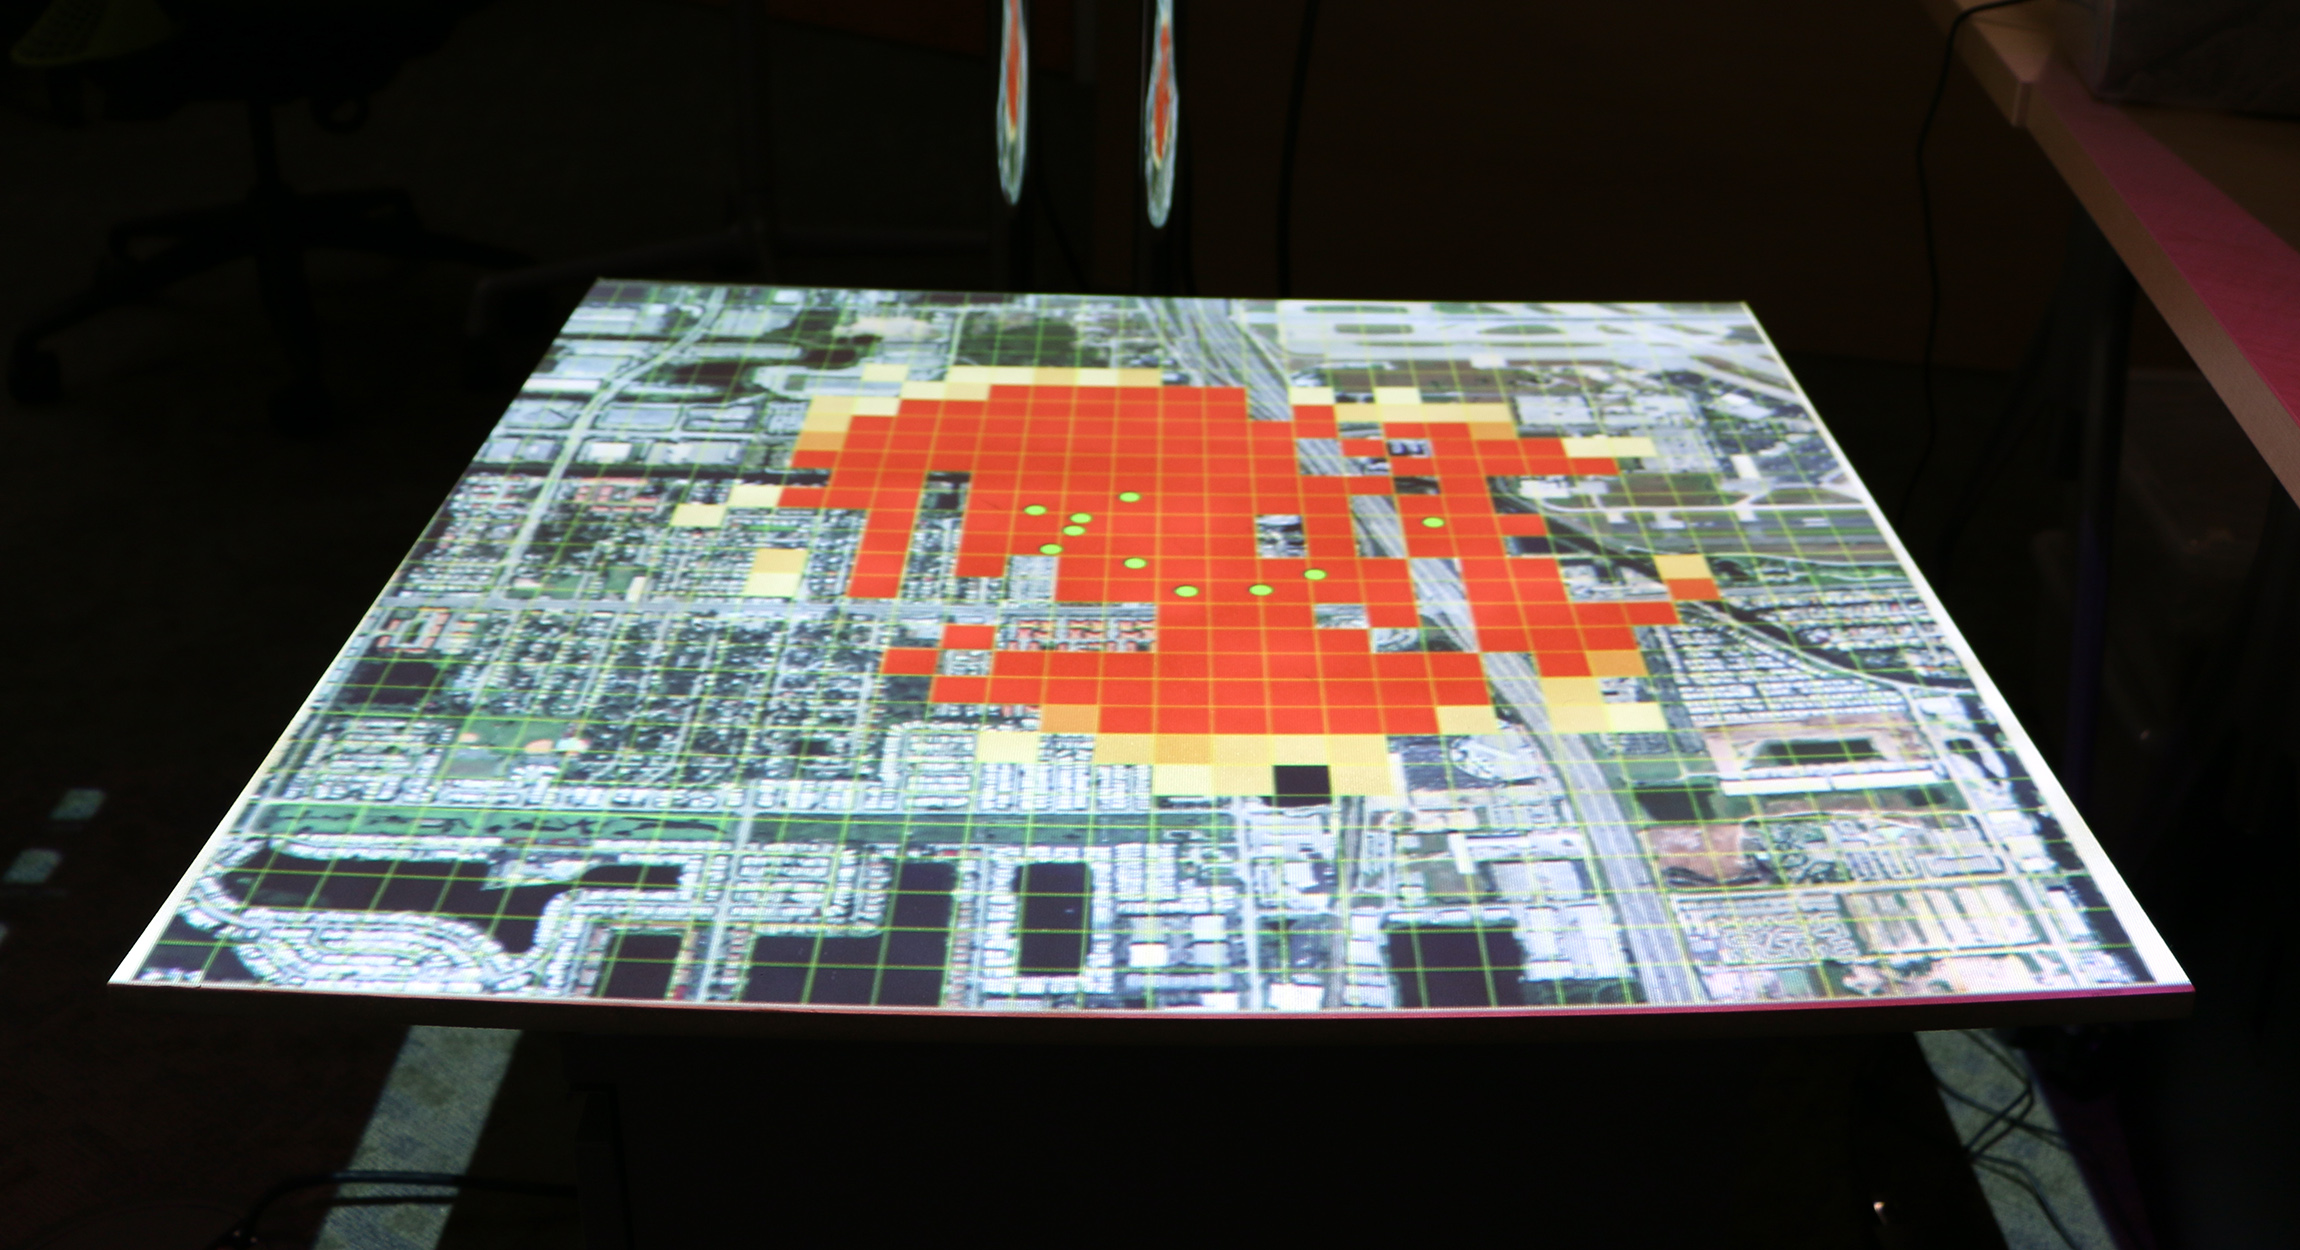
\includegraphics[width=0.3\textwidth]{images/termite_game_1.jpg}
		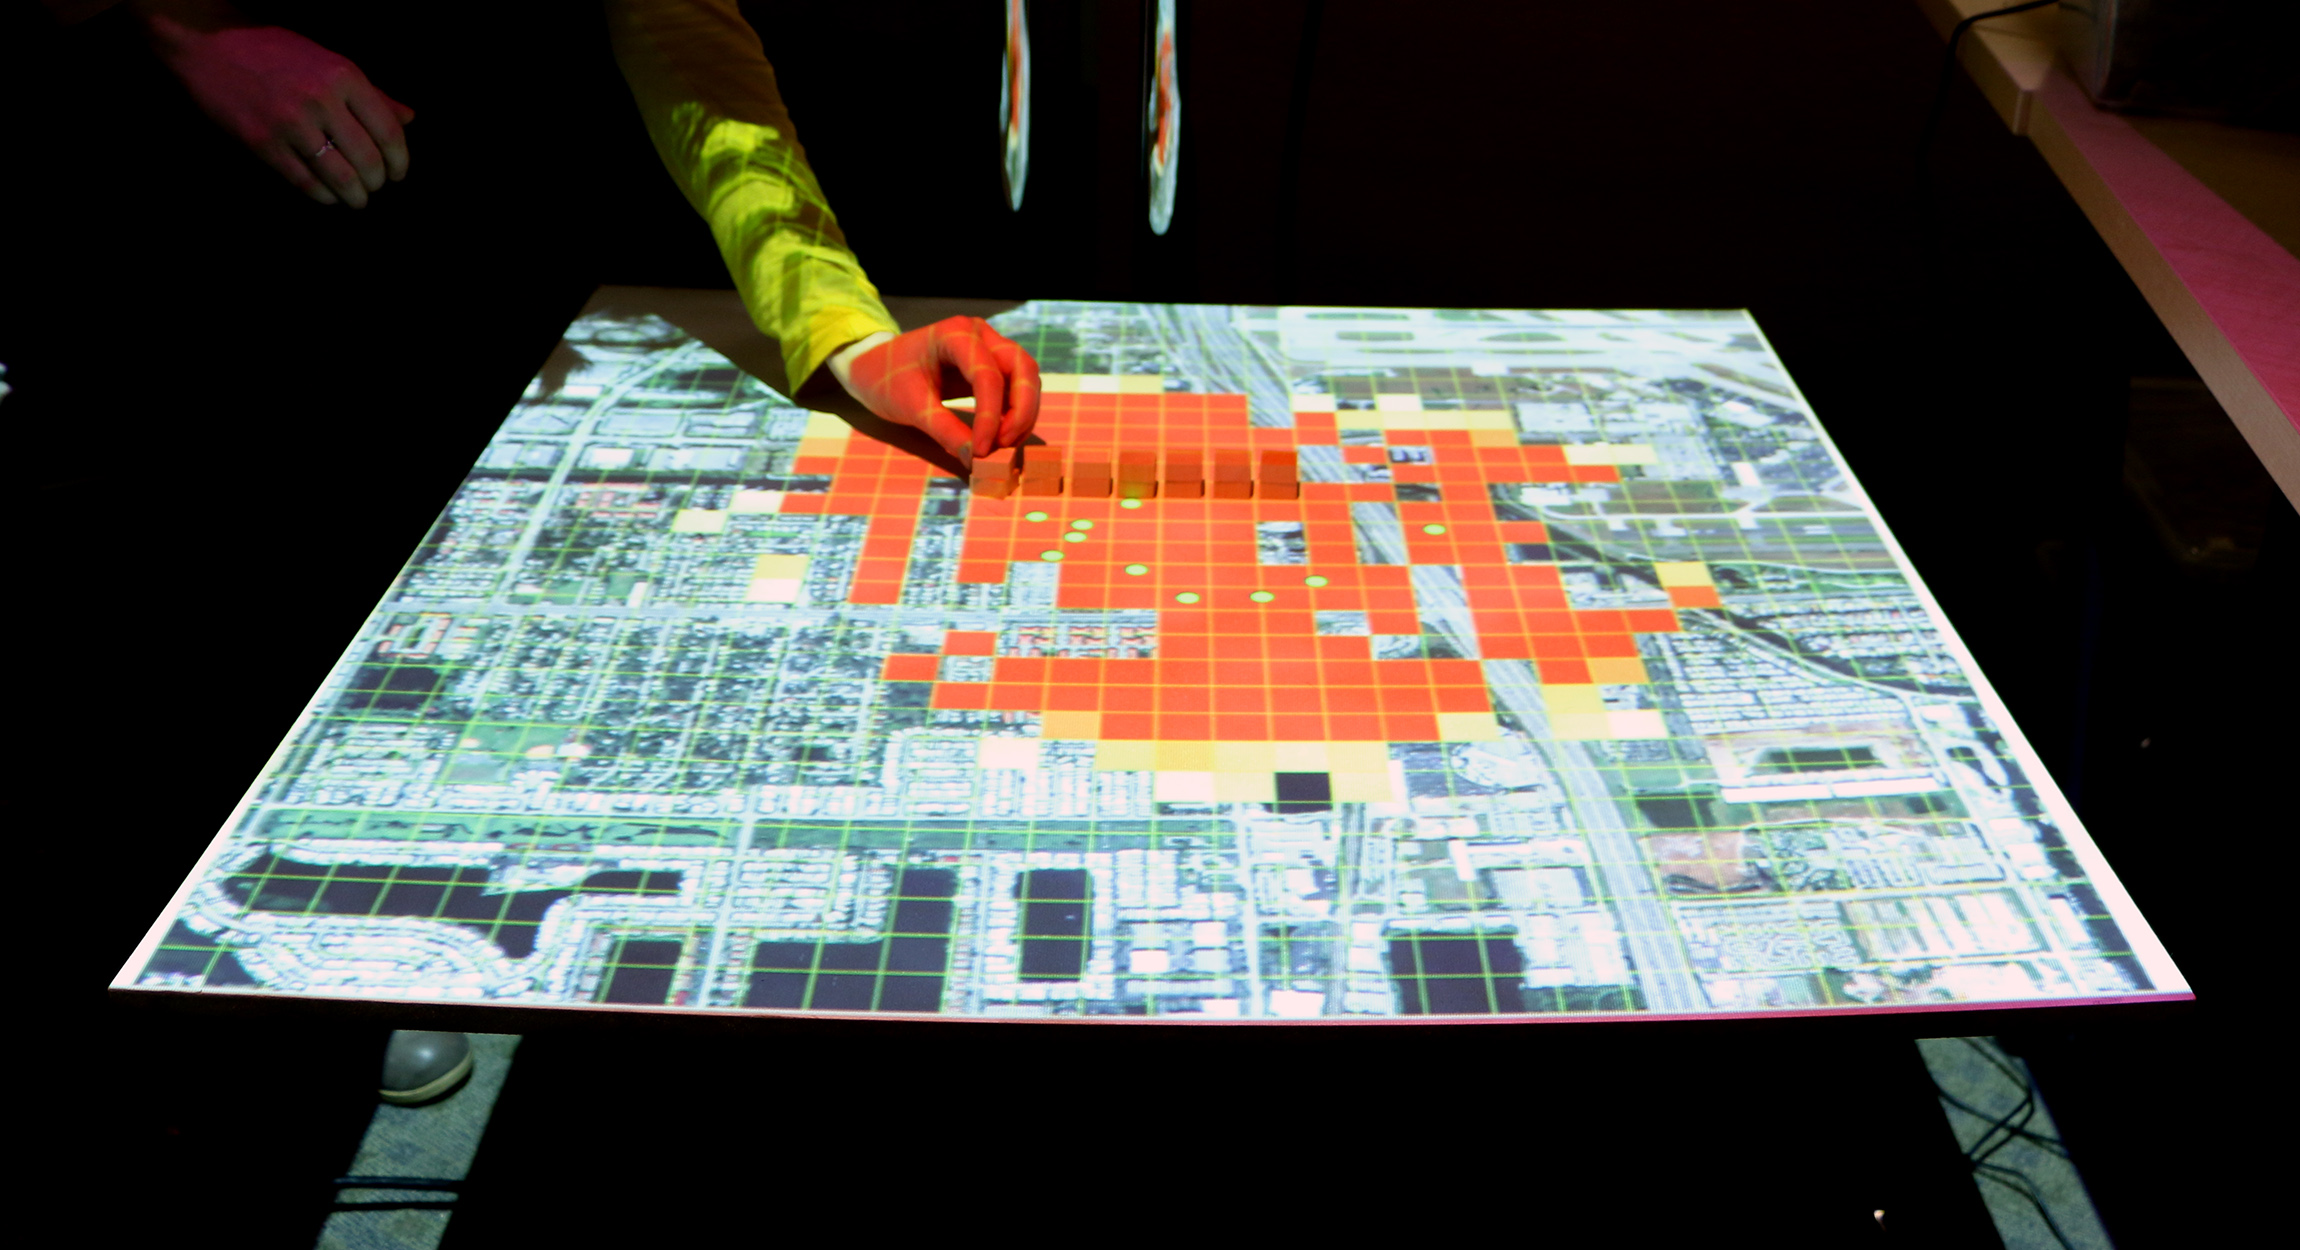
\includegraphics[width=0.3\textwidth]{images/termite_game_2.jpg}
		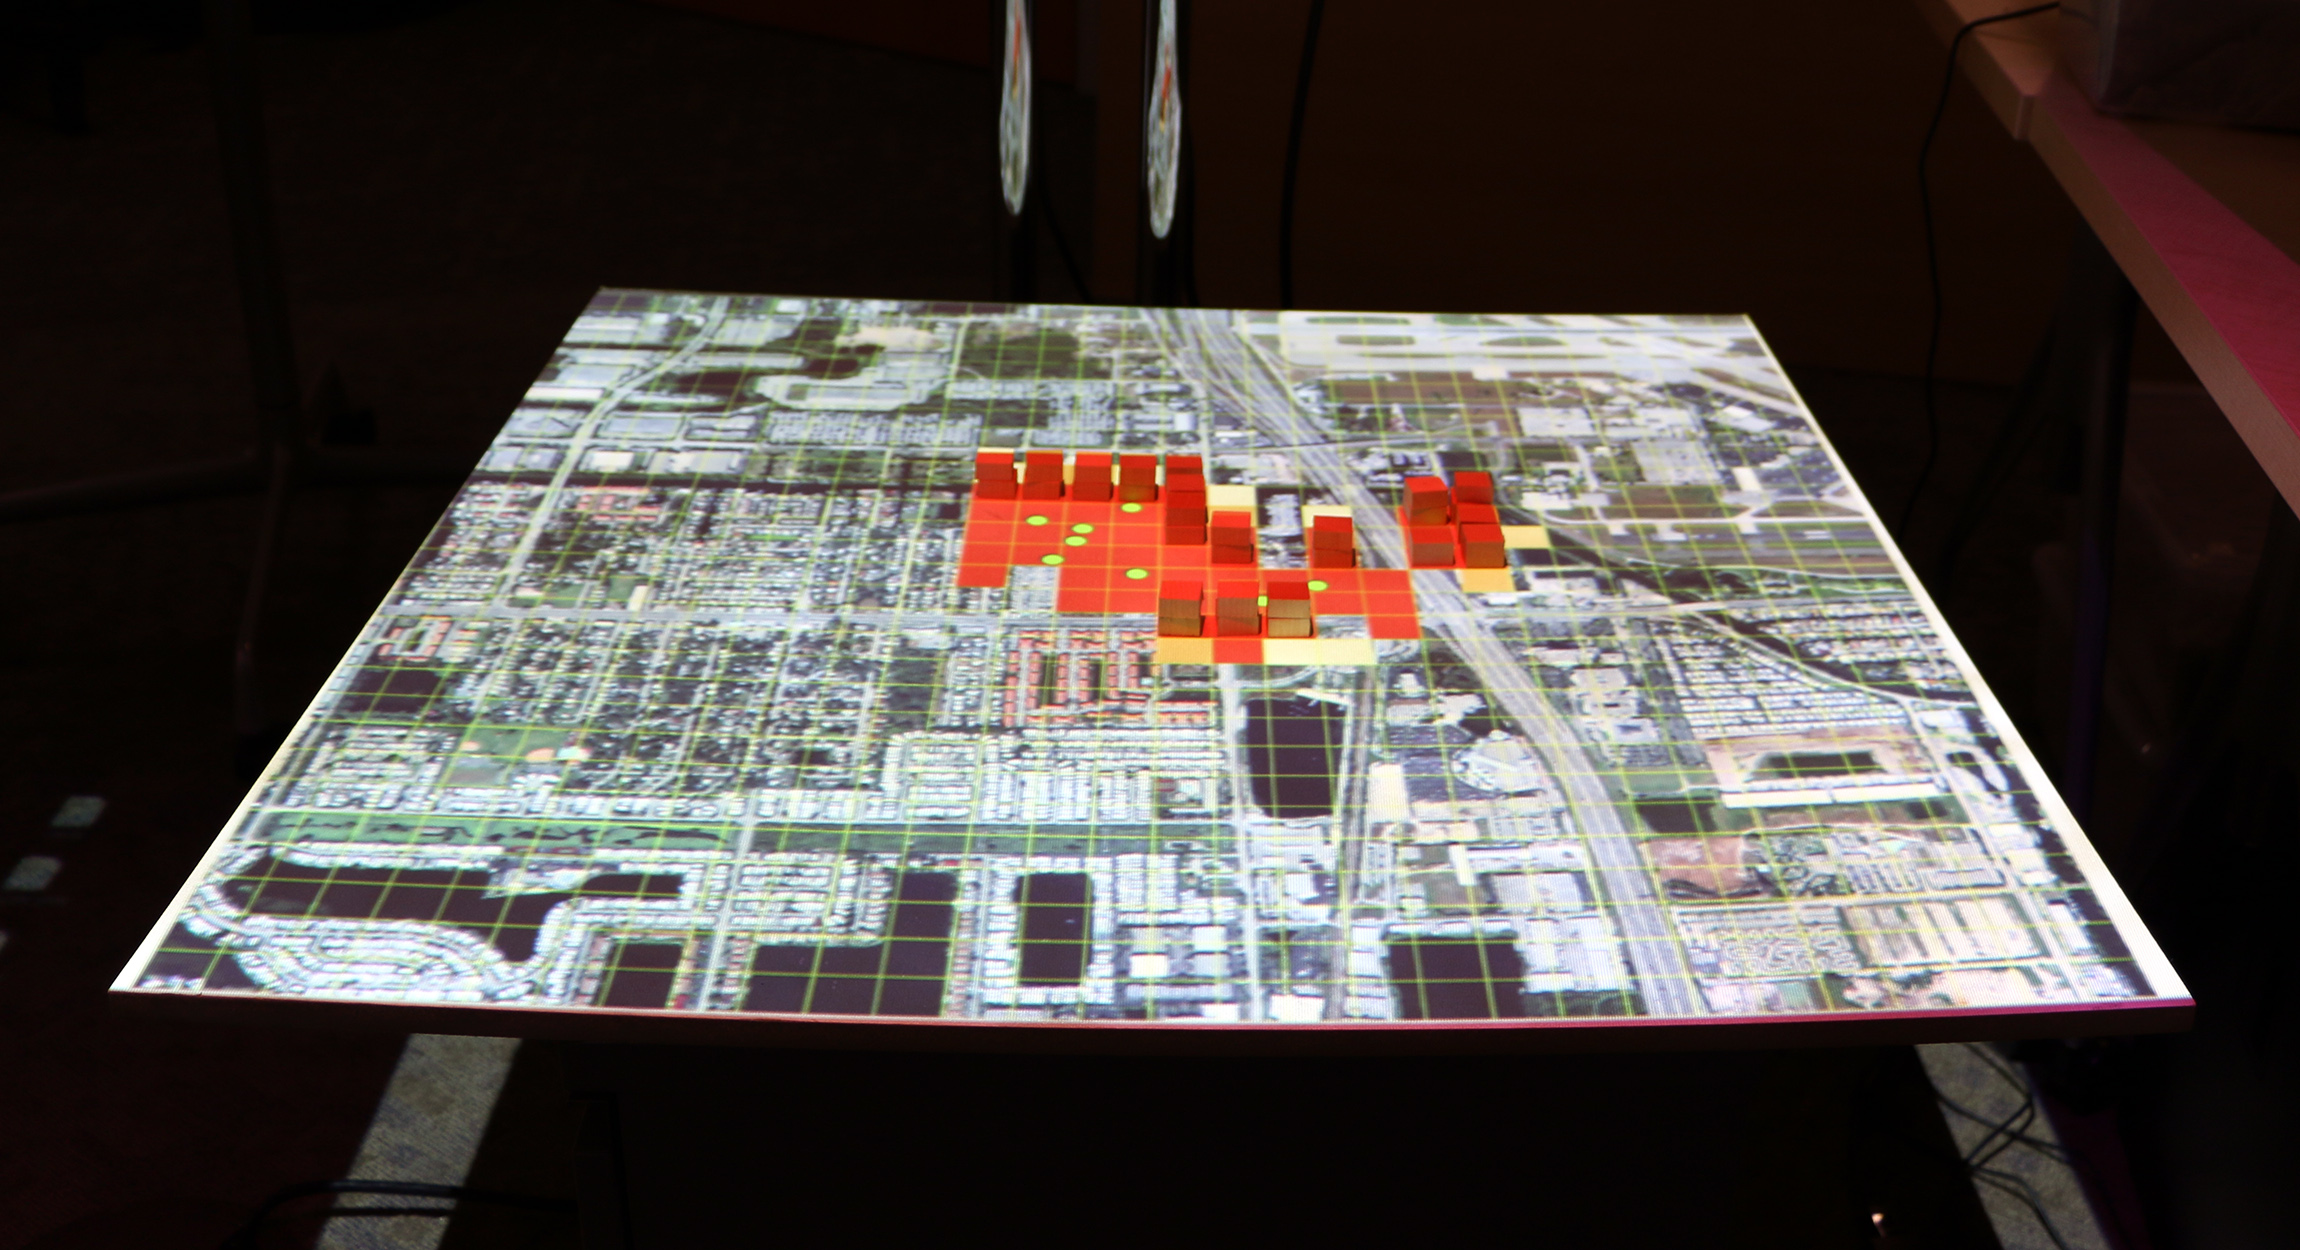
\includegraphics[width=0.3\textwidth]{images/termite_game_3.jpg}
	\caption{Managing the simulated spread of termites through a city with Tangible Landscape}
	\label{fig:termite_game}
\end{center}
\end{figure*}

\begin{figure*}[ht!]
\begin{center}
		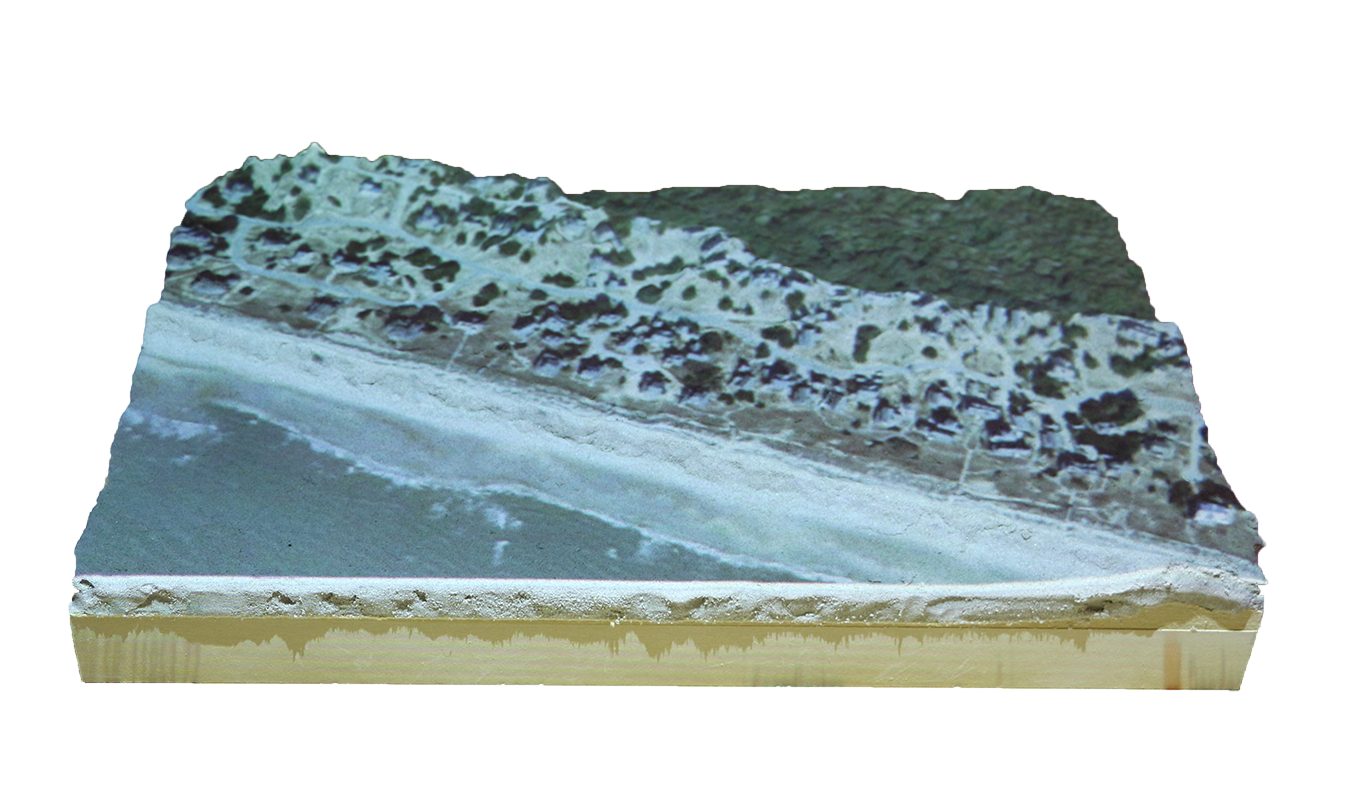
\includegraphics[width=0.3\textwidth]{images/tl_coastal_1s.png}
		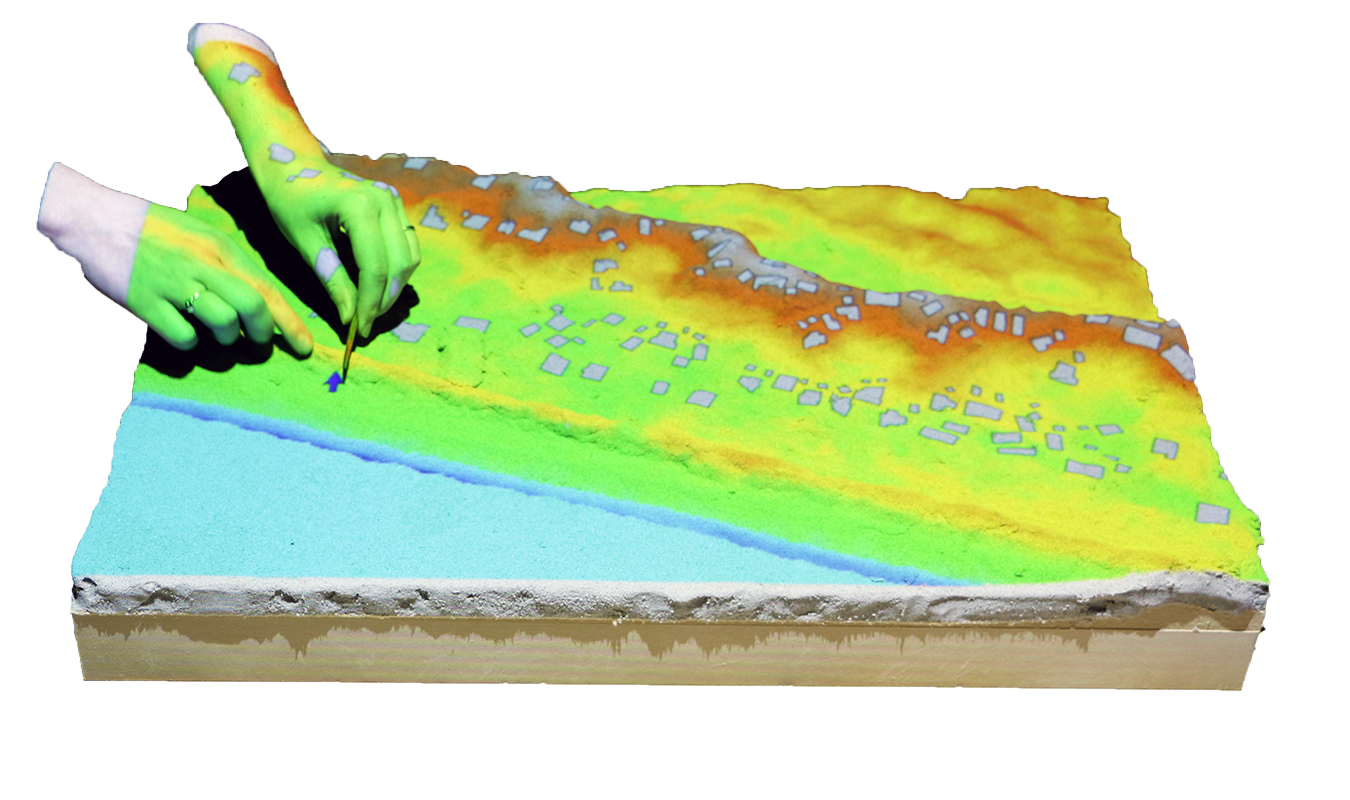
\includegraphics[width=0.3\textwidth]{images/tl_coastal_3s.png}
		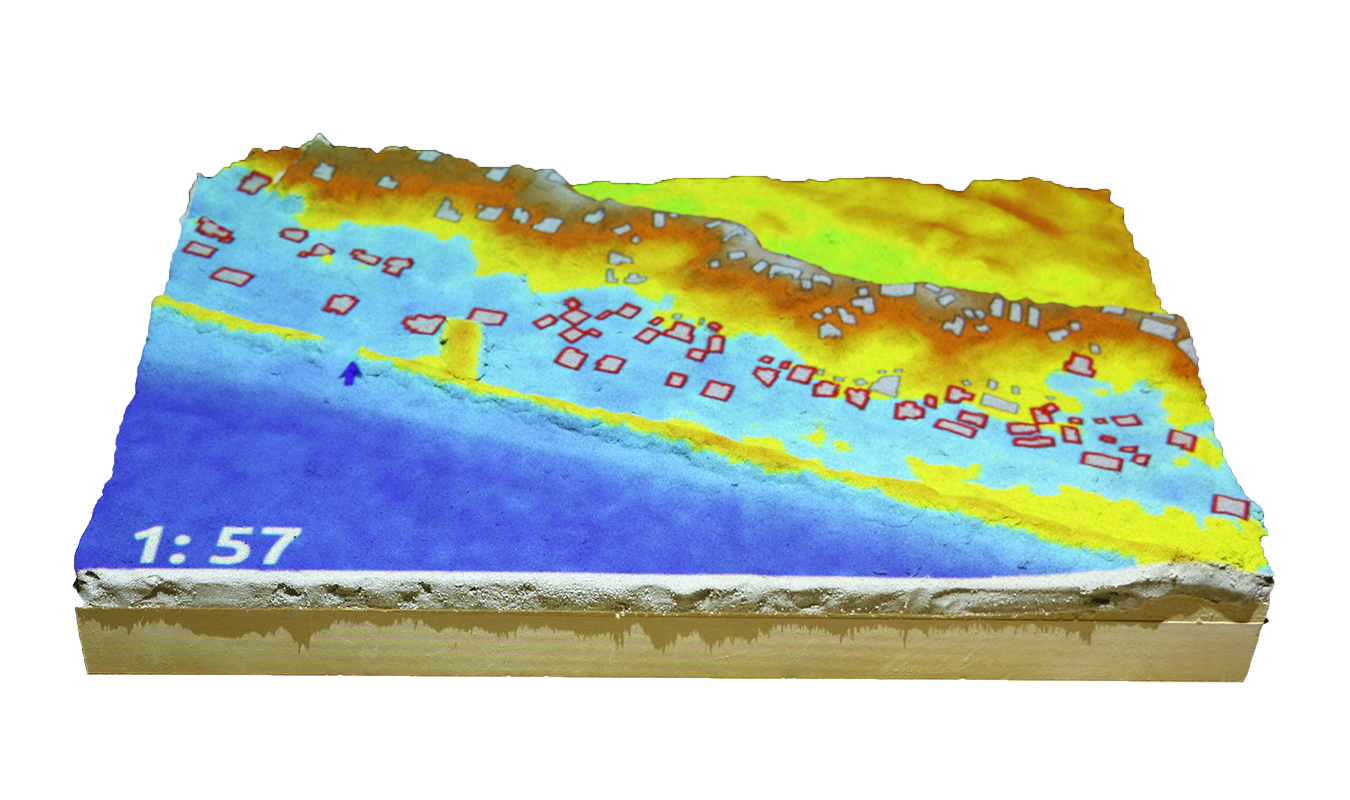
\includegraphics[width=0.3\textwidth]{images/tl_coastal_4s.png}
	\caption{...}
	\label{fig:coastal_game}
\end{center}
\end{figure*}

\section{Results}

\section{Discussion}

\subsection{Design guidelines}
\cite{Wilson2014}

\section{Future work}

% Cognitive science

% Real-time robotic fabrication
Figure~\ref{fig:system_schema_land} \ldots 

\begin{figure}%[h!]
\begin{center}
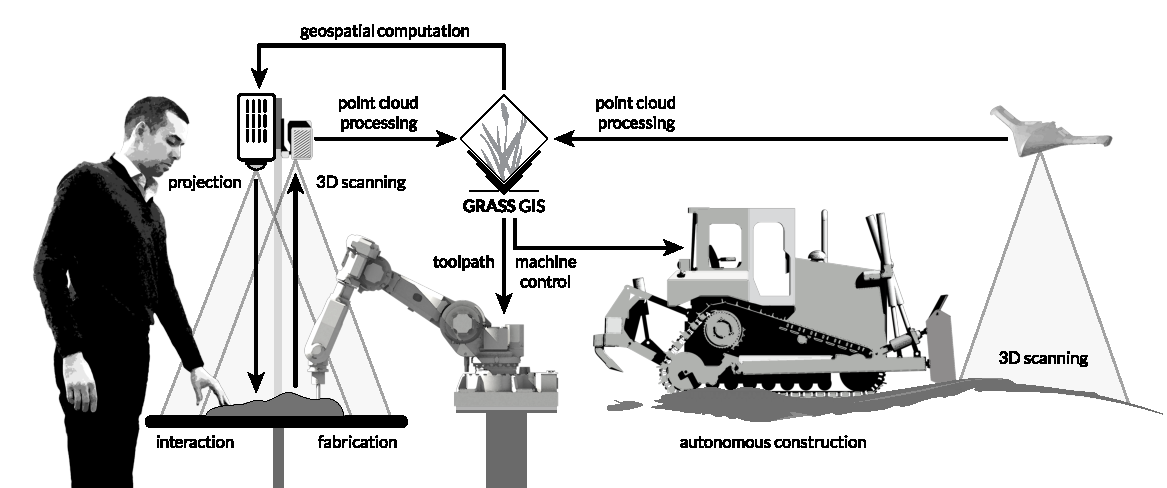
\includegraphics[width=\textwidth]{images/system_schema_land.pdf}
\caption{Tangible Landscape with robotic fabrication, robotic construction, and real-time field data}
\label{fig:system_schema_land}
\end{center}
\end{figure}

\section{Conclusion}

% Vision






%\section{...}
%% label
%\label{sec:examples}
%
%% Head 2
%\subsection{Head 2}
%
%% Head 3
%\subsubsection{Head 3}
%
%% Head 4
%\paragraph{Head 4}
%
%% quote
%\begin{quote}
%``\ldots".
%\end{quote}
%
%% itemize
%\begin{itemize}
%\item \ldots .
%\item \ldots .
%\item \ldots .
%\end{itemize}
%
%% footnote
%\ldots \footnote{...} 
%
%% enumerate
%\begin{enumerate}
%\item \ldots .
%\item \ldots . 
%\item \ldots .
%      \begin{enumerate}
%      \item \ldots .
%      \item \ldots .
%      \end{enumerate}
%\end{enumerate}
%
%% Enunciations
%\begin{definition}[...]...
%\end{definition}
%
%Table~\ref{tab:one}. 
%% Table
%\begin{table}%
%\tbl{...\label{tab:one}}{%
%\begin{tabular}{|l|l|}
%\hline
%...   & ...\\\hline
%...    & ...\\\hline
%\end{tabular}}
%\end{table}%

% Appendix
\appendix
\section*{APPENDIX}
\setcounter{section}{1}
In this appendix \ldots
\appendixhead{HARMON}

% Acknowledgments
\begin{acks}
\ldots
\end{acks}

% Bibliography
\bibliographystyle{ACM-Reference-Format-Journals}
\bibliography{tangible_topography.bib}

% History dates
%\received{}{}{}

% Electronic Appendix
\elecappendix

\medskip

\section{How-to-build}

\subsection{Hardware}
\begin{table}[hp!] \footnotesize \center
\caption{Hardware}
{\tabulinesep=1.2mm
\begin{tabu}{l l l}
\toprule
Type & Product & Cost\\
\midrule
Computer & System 76 Oryx Pro & \$1500\\
Projector & Optoma ML750 WXGA 700 DLP LED & \$500\\
3D sensor & Xbox One Kinect & \$100\\
& Kinect Adapter for Windows & \$50\\
Stand & Avenger 40-Inch C-Stand with Grip Kit & \$200\\
& Avenger 40-Inch C-Stand with Grip Kit & \$200\\
& Avenger F800 3-Inch Baby Wall Plate & \$10\\
& Avenger F800 3-Inch Baby Wall Plate & \$10\\
Peripherals & HDMI cable & \$10\\
& Extension cord & \$10\\
Modeling media & Waba Fun Kinetic Sand 11 Lbs & \$50\\
\bottomrule
\end{tabu}}
\label{table:hardware} 
\end{table}


\subsection{Data sources}
\begin{table}[hp!] \footnotesize \center
\caption{Data sources}
{\tabulinesep=1.2mm
\begin{tabu}{l l l}
\toprule
Data type & Data source & Link\\
\midrule
Lidar & United States Interagency Elevation Inventory & http://coast.noaa.gov/inventory/\\
& Earth Explorer & http://earthexplorer.usgs.gov/\\
& Digital Coast & http://coast.noaa.gov/dataviewer/\\
& Open Topography & http://www.opentopography.org/\\
Digital Elevation Models & National Elevation Dataset & http://viewer.nationalmap.gov/viewer/\\
Orthoimagery & USGS EROS Orthoimagery WMS & http://raster.nationalmap.gov/\\
\bottomrule
\end{tabu}}
\label{table:data_sources} 
\end{table}
























\end{document}



